%The tests were performed using the \gls{BUTPPG}~\cite{butppg}. In such a database, it was utilized a smartphone to record 48 \gls{ppg} signals of 12 \gls{sbjs} (\gls{sbjs}) index fingers, in such a manner that 3 records were extracted when the subject was sat down and a single record was extracted when he or she was walking \cite{butppg}. This database can be consumed through Physionet~\cite{physionet} interface via \texttt{wfdb} package. The proposed method was implemented in Python. Implementations of \gls{gaf}, \gls{mtf} and \gls{rp} were provided by PyTS \cite{pyts} library. The PyTorch library~\cite{pytorch} was used to perform the training and the classification operations. The models used in this study are listed in Table~\ref{tab:results} and provided by TorchVision. Hyper-parameters optimization was performed using the Optuna library~\cite{optuna}. For each model, 50 Optuna trials were performed for fitting and validating the \gls{ml} model with median pruner to avoid excessive computation of trial epochs that do not show hope of better results.

%After the optimization, the metrics of the best trial were evaluated in the testing dataset to assess the selected hyperparameters' process quality. With selected hyper-parameters for each \gls{ml} model in hands, the dataset was divided into folds using the cross-validation \gls{loso} re-sampling method, into pieces matching each of the 12 \gls{sbjs}. For each fold, the smaller split was used as the testing dataset for the evaluation of the model's metrics, while the bigger split was subdivided into the training dataset, of size 7 \gls{sbjs}; and into the validation dataset, of size 4 \gls{sbjs}. Applying such an experimental setup allowed the generation of results concerning the metrics present in Table~\ref{tab:results}, where, for each projection method, all models were seen as samples of a statistics population possessing 5 values corresponding to the mean of all 12 folds of each metric.

% The hyper-parameters selection can be a computationally expensive process, considering large sets of possible parameters to be searched exhaustively. Hence, Optuna, a hyper-parameter optimization framework based on heuristic search with pruning \cite{optuna}, was used. But, before selecting such parameters, it was needed to separate the dataset in train, with 7 \gls{sbjs}; validation, with 2 \gls{sbjs}; and test, with 3 \gls{sbjs}; splits.  Later, it was optimized, in 50 Optuna trials, using the train dataset for fitting the \gls{ml} model and the validation dataset for evaluating the objective function value. Furthermore, it was used Optuna's median pruner to avoid excessive computation of trial epochs that do not show hope of better results, if compared to previous trials. Such an optimization process allowed to find the set of best hyper-parameters for each model, which, in this case, contain only the learning rate. 

%In order to evaluate those projection methods, the following metrics were considered accuracy score, the proportion of hits $Accuracy = \frac{(TP+TN)}{TP+TN+FP+FN}$; precision score, the proportion of correct positive guesses, $Precision = \frac{TP}{TP+FP}$; recall score, the proportion of found positive samples, $Recall = \frac{TP}{TP+FN}$; and F1 score, the harmonic mean between the precision score and the recall score, $F1 = 2 \cdot \frac{Precision \cdot Recall}{Precision + Recall}$. Additionally, it was measured the Cohen Kappa score, the degree of agreement of annotators for a classification problem, $CohenKappa = 1-\frac{1-p_o}{1-p_e}$, where $p_o$ is the proportion of observed concordance and $p_e$ is the probability of concordance between all annotators. In the supervised binary classification domain, only two annotators, corresponding to the predicted and the real labels, and two classes, corresponding to positive or negative, are considered, in a manner that the confusion matrix can be used directly to evaluate the score, by the formula $CohenKappa=\frac{2\cdot (TP\cdot TN - FP \cdot FN)}{(TP+FP)\cdot(FP+TN)+(TP+FN)\cdot(FN+TN)}$.

% Those metrics were evaluated for 70 \gls{ml} models implemented in \href{https://pytorch.org/}{PyTorch}, the ones listed on Table~ \ref{tab:results}
% For such networks, the same experiment framework was applied, highlighting three major process blocks: dataset construction, when the database was loaded and transformed; hyperparameters selection, when, for each \gls{ml} model, a search was done to try to find the set of its best hyperparameters for the built dataset; and projection metrics evaluation, when each model, in conjunction with its set of best hyper-parameters found, was tested, generating the metrics present in this article. %(the framework is shown in figure \ref{figure:framework})
% Also, hyper-parameters selection and projections evaluation apply training and testing cycles.  To clarify those processes, they will be described in detail in the following sections.


%\begin{figure*}[t]
%    \centering
%    \includegraphics[width=\linewidth]{imgs/framework2.pdf}
%    \caption{Flowchart representing the experimental framework. Gray elements are entities, while blue elements are processes.}
%    \label{figure:framework}
%\end{figure*}

% \subsection{Training and Testing}

% Machine learning tasks involve 2 main steps: training and testing. Such a format was applied several times on the hyper-parameters selection process, for testing certain sets of hyper-parameters; and the projections evaluation process, for evaluating the model and its set of hyper-parameters efficiency. That core task was done using \href{https://pytorch.org/}{PyTorch} python library, which automatically computes the gradients based on the user's implementation \cite{pytorch}. Also, it allows parallel GPU processing to be done, by applying tensor-based operations to batches of the dataset, which size used in this experiment was the whole dataset. 

% The training process parameters also involve an optimizer and and loss function. The optimizer algorithm to be used was Adam\cite{adam}, while the Cross-Entropy Loss function was used, %\cite{cross-entropy-loss} 
% both implemented in \href{https://pytorch.org/}{PyTorch}. Moreover, the training process needs to stop at some point, fact that was done using an early stopping approach, computing the median absolute deviation, deviation metric robust to outliers, %\cite{?}
% of a window of the last 10 loss function values on the validation dataset, stopping the training process when such windows converge to, at least, a deviation of value 1. When the training process stopped, the best result found was chosen.

% \subsection{Dataset construction}

% In order to provide data to train and test \gls{ml} models, the Brno University of Technology Smartphone PPG Database was used as a starting point. In such a database, it was utilized a smartphone to record 48 \gls{ppg} signals of 12 \gls{sbjs} (\gls{sbjs}) index fingers, in such a manner that 3 records were extracted when the subject was sat down and a single record was extracted when he or she was walking \cite{butppg}. Additionally, other refinement procedures were done to perfect that database, such as cropping 20 seconds of the recording, leaving the middle 10 seconds intact\cite{butppg}. And, finally, the database is publicly available on Physionet through the link \url{https://physionet.org/content/butppg/1.0.0/}. 

% However, the database is in \gls{wfdb} format \cite{butppg}, one dimensional signal format in function of time, %\cite{wfdb}
% letting yet to be done the application of projection methods. For such purpose, PyTS was used, a Python package developed for time series classification, containing the desired projection algorithms, \gls{gaf}, \gls{mtf} and \gls{rp} \cite{pyts}, with its implementations of PyTS version 0.13.0 stored in \href{https://zenodo.org/}{Zenodo} repository \cite{pyts-v0.13.0}.
    
% With such a package, it was possible to produce a dataset containing all projections as 2D images with 3 channels with shape $3 \times siglen^2 \times siglen^2$, where $siglen$ is the signal length. For each projection, its matrix was repeated on every channel of the image, while the \gls{PM} filled every channel with each of the 3 mentioned projections. Finally, it was necessary to resize every image for each \gls{ml} model input shape, for such purpose that it was used \href{https://pytorch.org/}{PyTorch} resize transform with bi-linear interpolation. After those procedures, the dataset was ready for the following processes, as the hyper-parameters selection.

% \subsection{Hyper-parameters selection}

% The hyper-parameters selection can be a computationally expensive process, considering large sets of possible parameters to be searched exhaustively. Hence, Optuna, a hyper-parameter optimization framework based on heuristic search with pruning \cite{optuna}, was used. But, before selecting such parameters, it was needed to separate the dataset in train, with 7 \gls{sbjs}; validation, with 2 \gls{sbjs}; and test, with 3 \gls{sbjs}; splits.  Later, it was optimized, in 50 Optuna trials, using the train dataset for fitting the \gls{ml} model and the validation dataset for evaluating the objective function value. Furthermore, it was used Optuna's median pruner to avoid excessive computation of trial epochs that do not show hope of better results, if compared to previous trials. Such an optimization process allowed to find the set of best hyper-parameters for each model, which, in this case, contain only the learning rate. 

%\subsection{Projection Metrics Evaluation}

%After the optimization, the metrics of the best trial were evaluated in the test dataset to assess the selected hyperparameters' process quality. With selected hyper-parameters for each \gls{ml} model in hands, the dataset was divided into folds using the cross-validation \gls{loso} re-sampling method, into pieces matching each of the 12 \gls{sbjs}. For each fold, the left split was used as the test dataset for the evaluation of the model's metrics, while the other split was subdivided into the train dataset, of size 7 \gls{sbjs}; and into the valid dataset, of size 4 \gls{sbjs}. Applying such an experimental setup allowed to generate results with respect to the before-mentioned metrics, where, for each projection method, all models are seen as samples of a statistics population possessing 5 values corresponding to the metrics.

%Figure~\ref{fig:boxplots} depicts presents the boxplot of Accuracy, F1-score, Precision, Recall, and Cohen's Kappa distributions for different \glspl{CV} models tested on the \gls{BUTPPG} database. From these graphs, we can notice that, for the recall score, all projections are very equated. Moreover, it is noticeable that \gls{rp} and the proposed \gls{PM} have improved performances when compared with other \gls{mtf} and \gls{gaf} projections, especially when we observe the minimum, maximum, and the first quartiles of distributions, presented in Table~\ref{tab:boxplots}. From this table, we can perceive, at first glance, that the \gls{rp} and the \gls{PM} are generally superior methods if compared with the other two. In fact, \gls{rp} and \gls{PM} first quartiles are greater than \gls{gaf} and \gls{mtf} third quartiles considering all metrics except Recall Score, which shows that 75\% of samples in \gls{rp} and \gls{PM} are generally greater than 75\% of samples in \gls{gaf} and \gls{mtf}. The detailed performance of the points in the distributions considered in Figure~\ref{fig:boxplots} is depicted per model in Table~\ref{tab:results}.

%\input{tables/results}

% Each of the 4 populations produced box plots shown in figure \ref{fig:boxplots}, allowing, at first glance, to see the Recurrence Plot and the \gls{PM} as generally superior methods if compared with the other two. In fact, \gls{rp} and P\gls{PM} first quartiles are greater than \gls{gaf} and \gls{mtf} third quartiles considering all metrics except Recall Score, what shows that 75\% of samples in \gls{rp} and \gls{PM} are generally greater than 75\% of samples in \gls{gaf} and \gls{mtf}.    %TODO: falar do Cohen Cappa Score 

This chapter first presents the experimental setup. Then, it exposes and discusses the experimental results. Finally, it investigates the experiments limitations. 

\section{Experimental Setup}

This section discusses the experimental setup, analyzing elements used in the experiments, such as datasets, programming libraries and predictive models. Additionally, it clarifies metrics to be evaluated and approaches to measure them.  

\subsection{The dataset}

As for every machine learning task, we need a dataset to provide data to feed the predictive models for their parameters fitting, molding them to the domain of the specific task. In this work, the task of assessing the quality of the signal is a supervised classification problem, that is, can be described as the problem of finding a function that best defines a predefined set of pairs of variables and label, $(X,y)$. In this scope, the pair corresponds to the signal itself mapped to its quality label, ``Good'' or ``Bad''. For the purpose of training the predictive methods and evaluating their ability to fit to the problem of classifying the quality of heartbeat time series, the \gls{BUTPPG}~\cite{butppg} dataset was employed.

%
\begin{figure}
	\begin{tabular}{cc}
		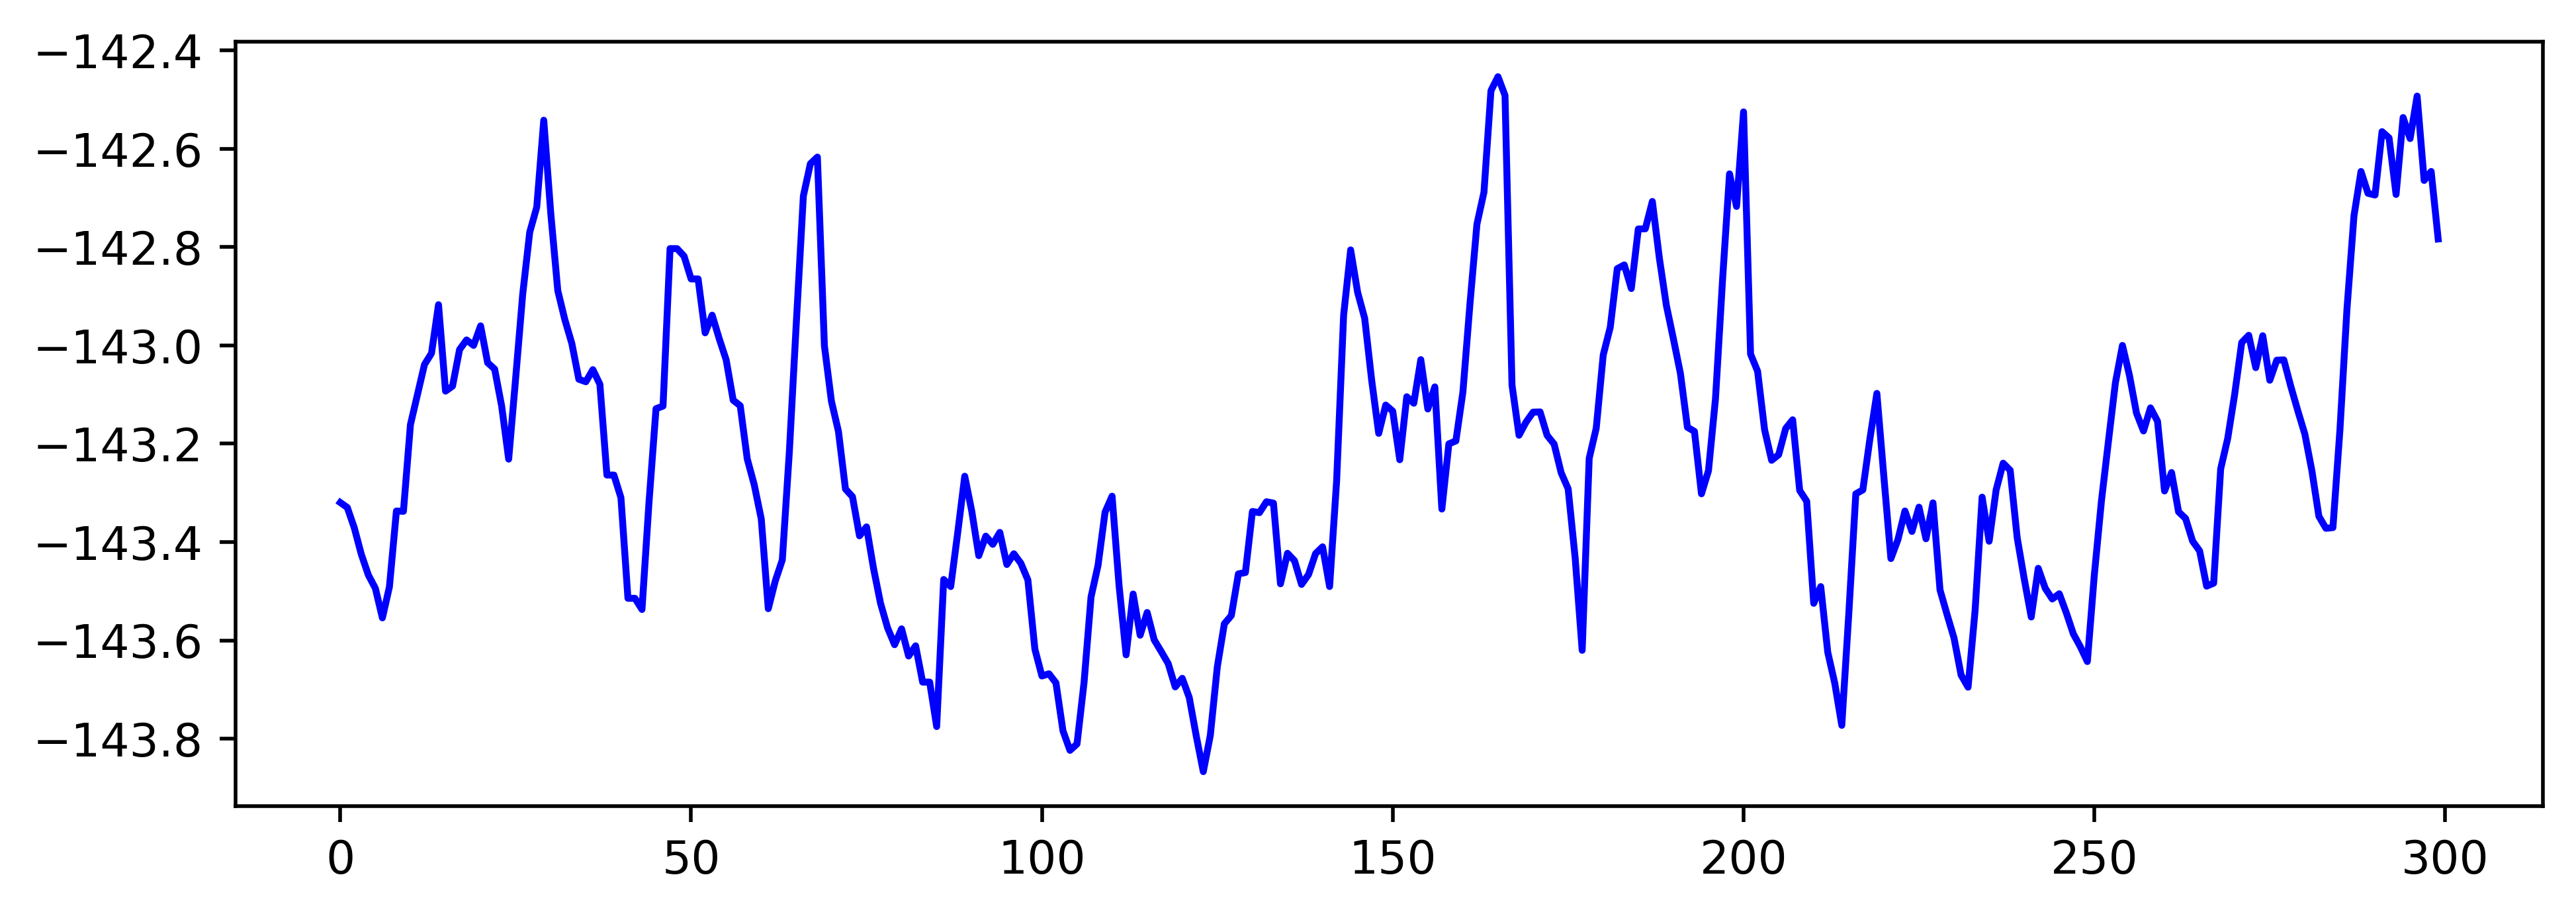
\includegraphics[width=0.45\linewidth]{img/samples/butppg_111001.png} 
			& 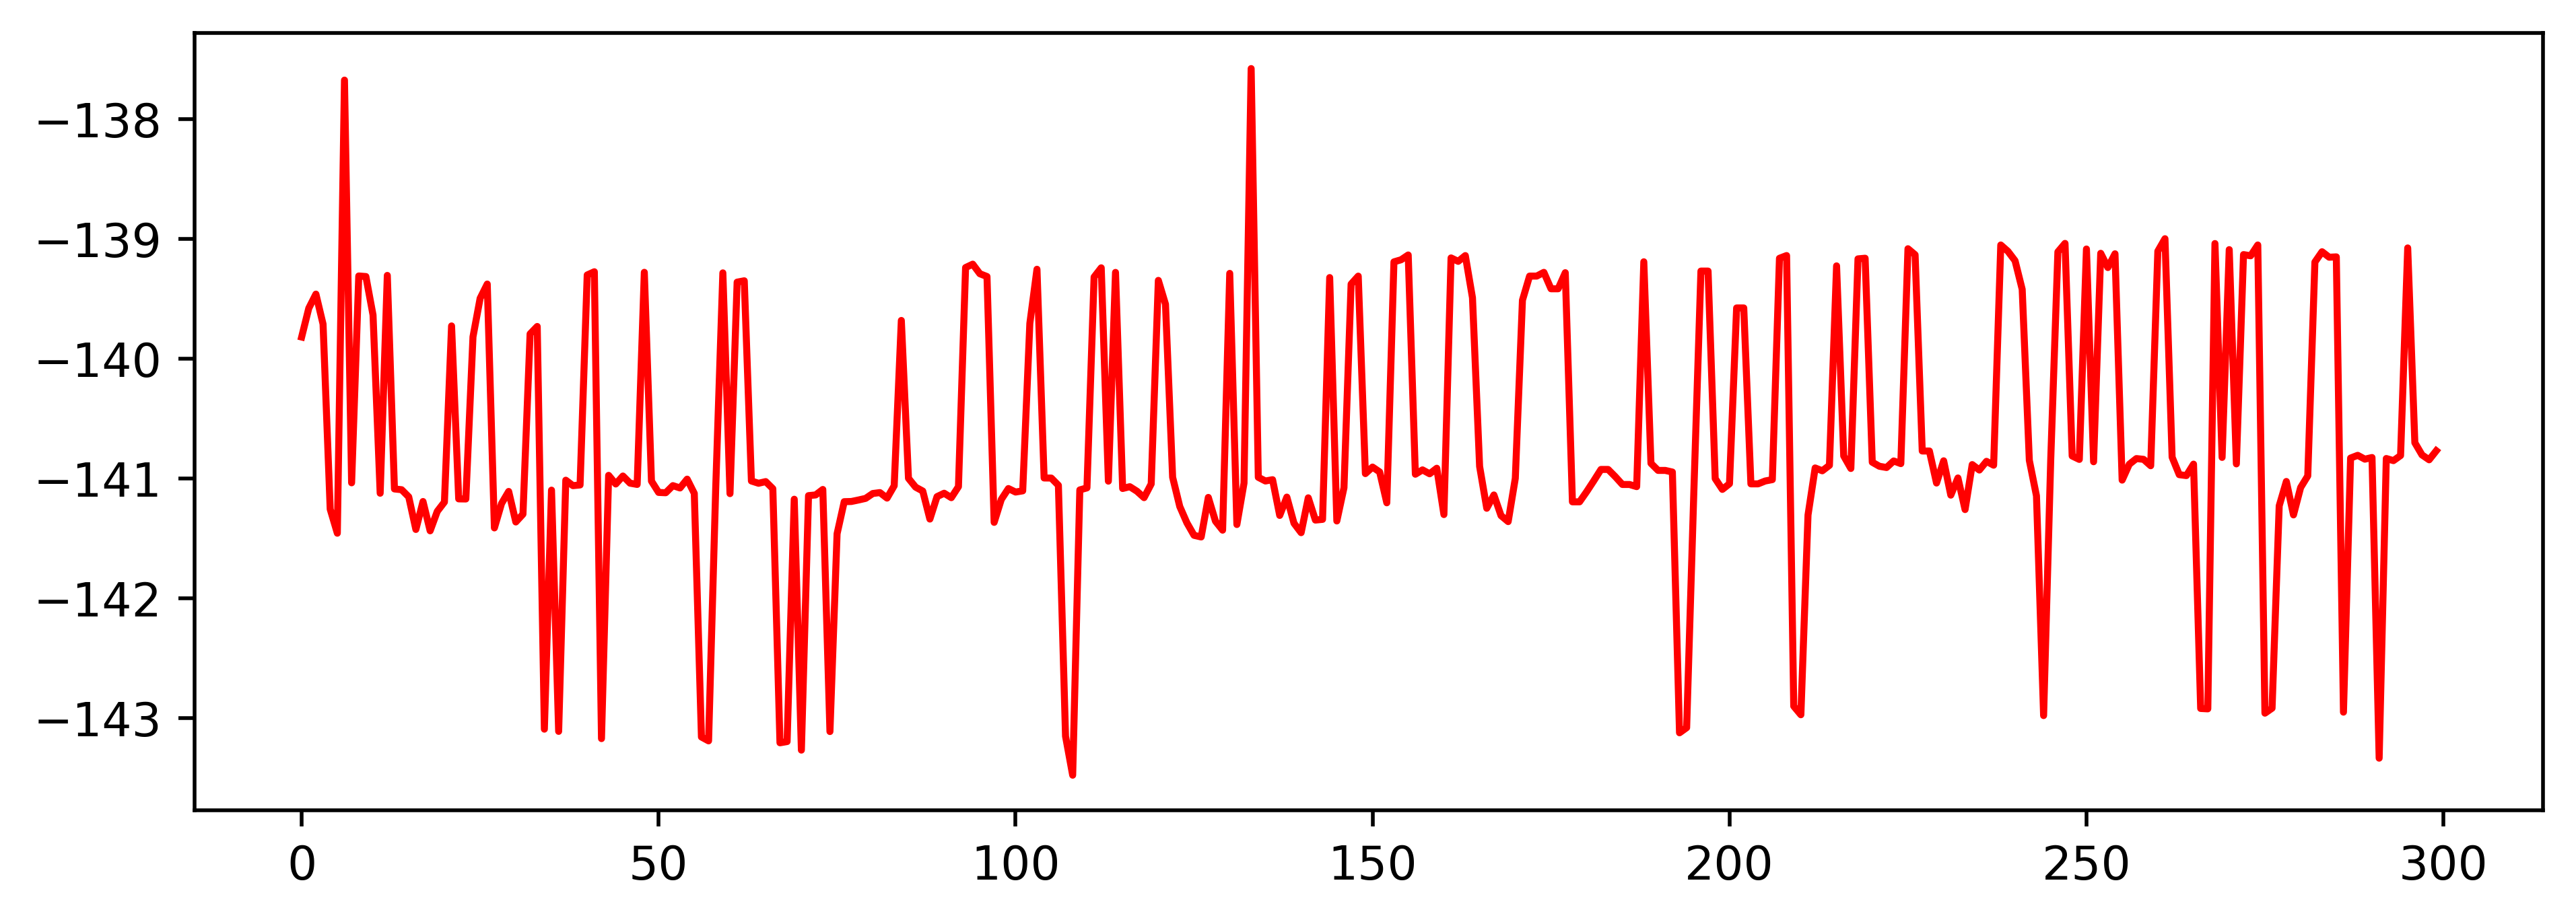
\includegraphics[width=0.45\linewidth]{img/samples/butppg_111003.png} \\
		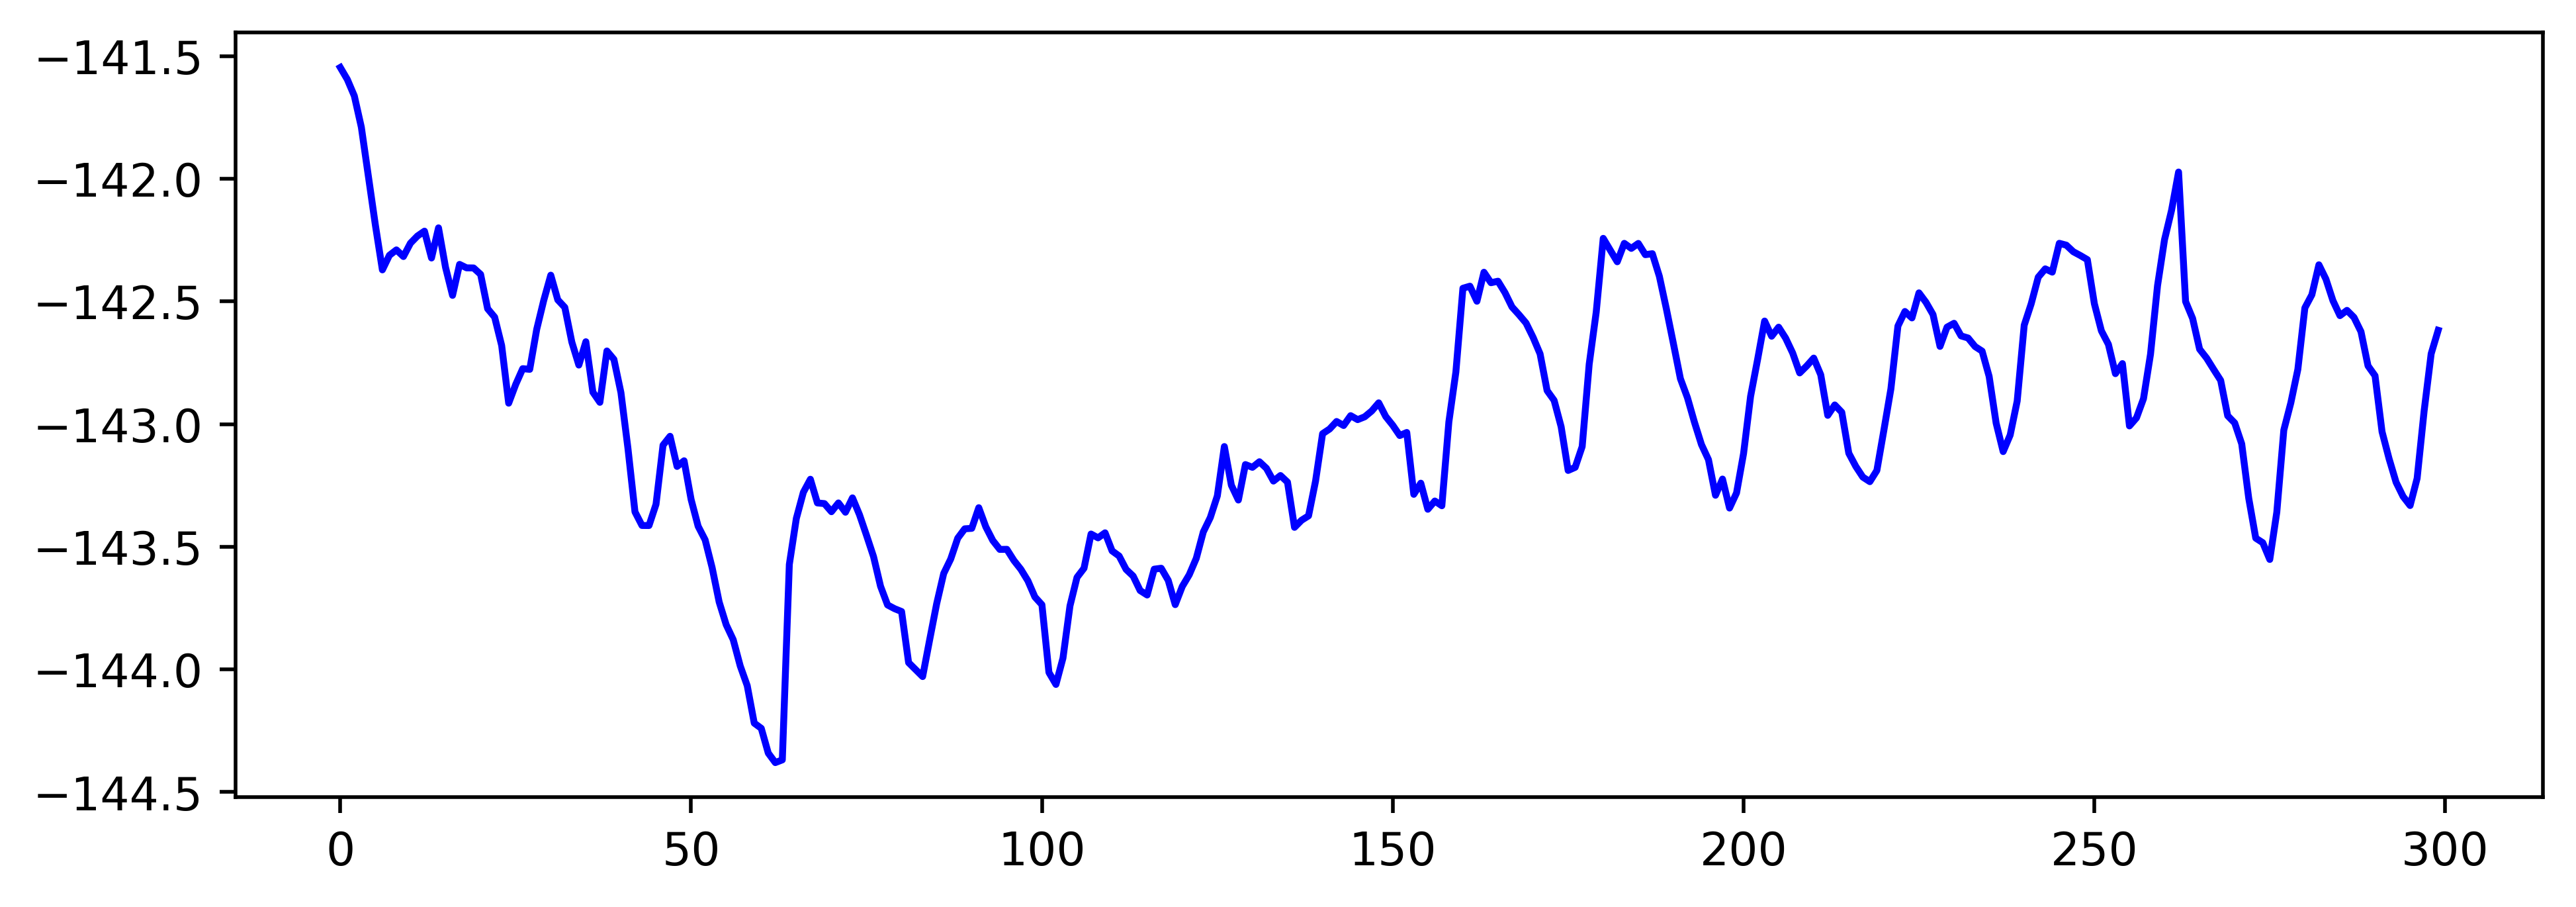
\includegraphics[width=0.45\linewidth]{img/samples/butppg_111002.png} 
			& 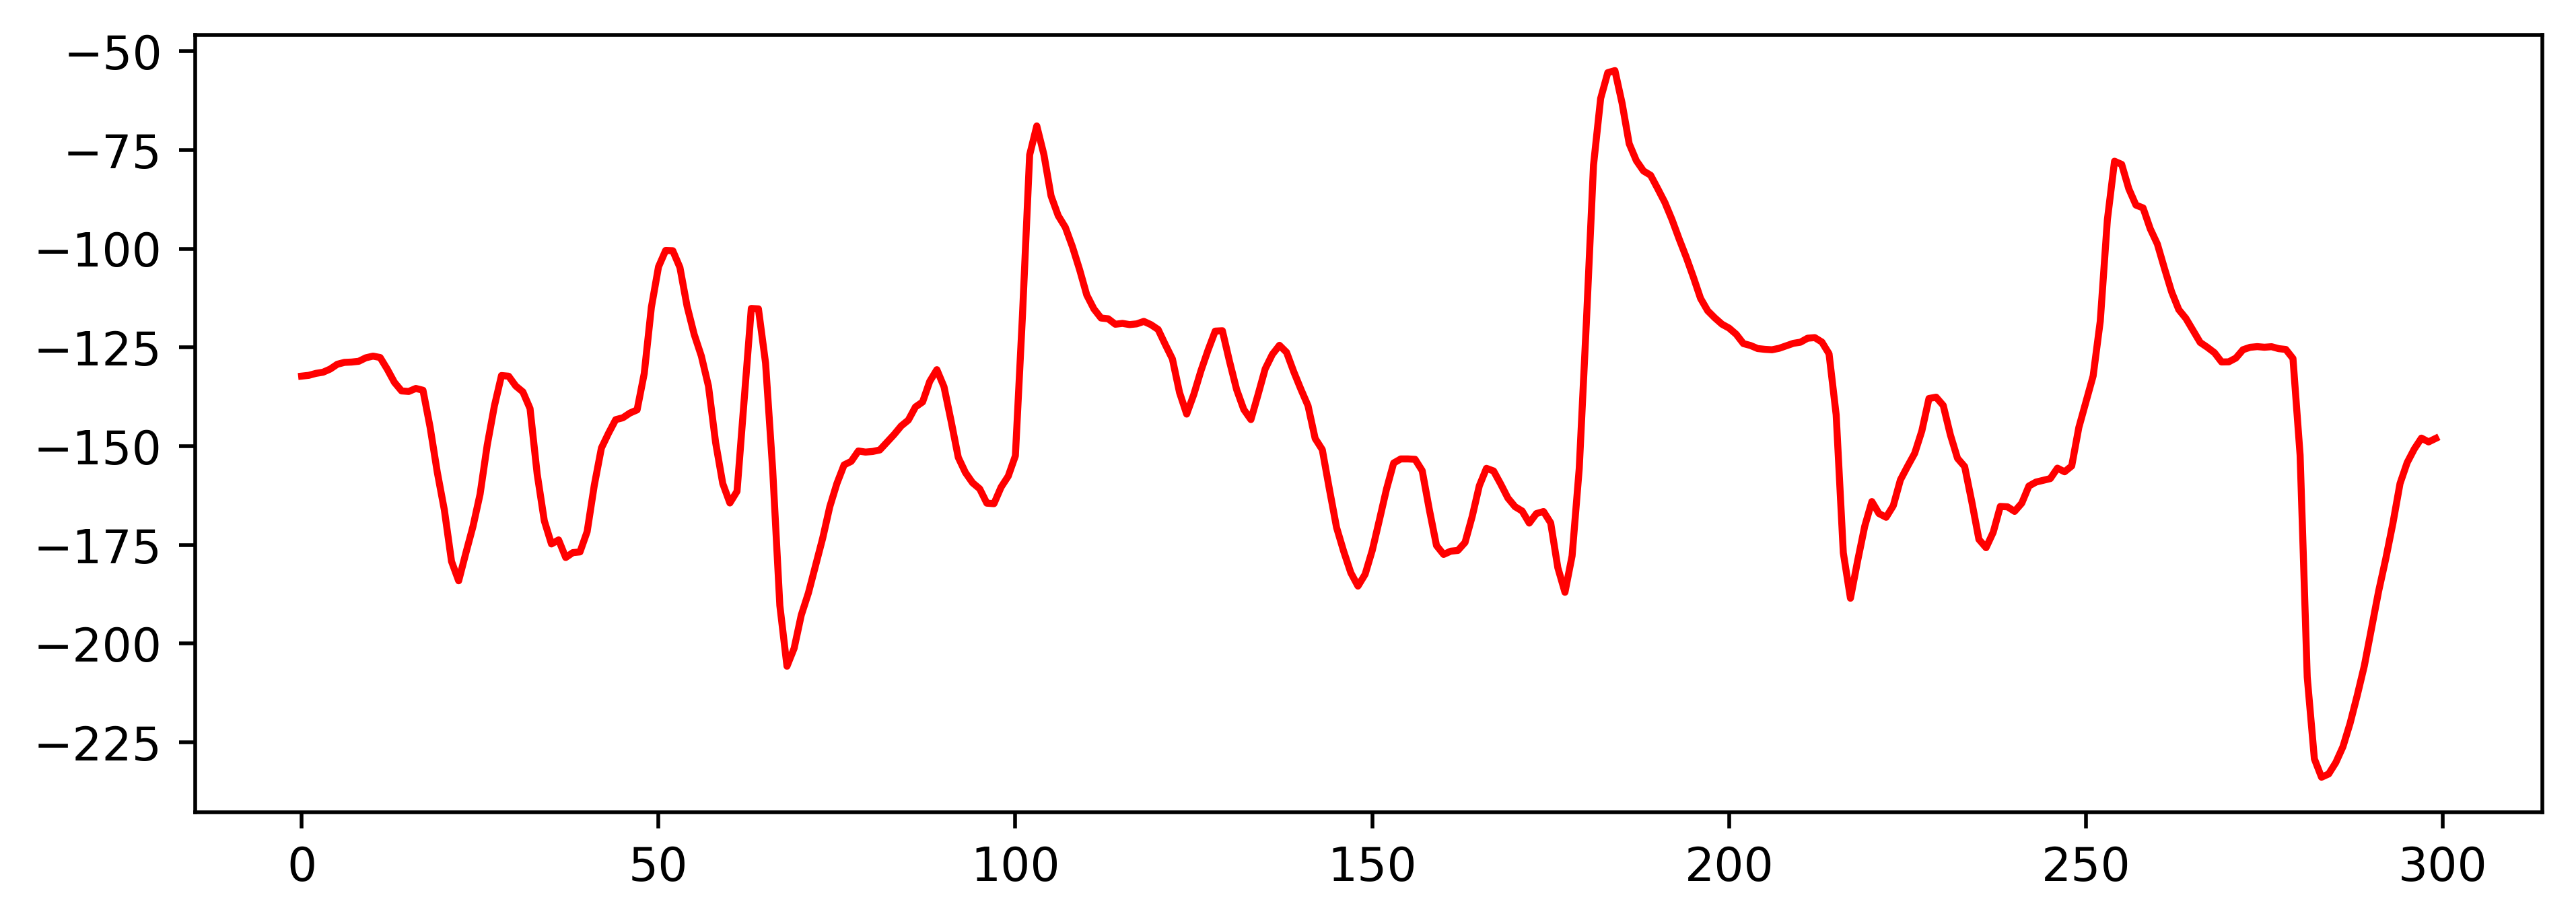
\includegraphics[width=0.45\linewidth]{img/samples/butppg_111004.png} \\
	\end{tabular}
	\caption{Samples of the four signals of the subject with id equal to 11 (where the first subject has id 0). The ``Good'' signals color is blue, while the ``Bad'' signals are red. In those graphs, the vertical dimension is the average of all pixels intensity in a frame, while the horizontal dimension is the time instant in frames. Notice that, since those records are 10 seconds long, it's implied that the sampling frequency is 30 Hz.}
	\label{fig:butppg_samples}
\end{figure}


The \gls{BUTPPG} is a publicly available database produced by the Department of Biomedical Engineering of the the Brno University of Technology. It contains samples of \gls{PPG} signals, its quality labels and its heat rate estimations. Those signals were extracted using a low-cost method: recording with the camera of a smartphone. To be more precise, the researchers recorded the subject's index finger, covering the lens of the camera and its \gls{LED} light. Then, they measured, for each video frame, the average of the intensities of the red channel of every image pixel, resulting in a time series of averages. Finally, they inverted the signal. %The Figure \ref{fig:butppg_samples} shows examples of the results of such a sequence of procedures.  

They done this method of obtaining \gls{PPG} signals  48 times, ammount distributed equally between 12 subjects. That is, for each subject, they did 4 measurements. Moreover, they did those recordings in two possible situations: one which the subject sat down and stayed static, case which the quality label ``Good'' was probable; and other in which the subject walked, hence, case likely to be a ``Bad'' recording. That distinction is relevant, since the walking situation occurred only 1 time for each subject, biasing the labels proportion to be nearly 25\% of ``Bad'' ones. Therefore, this dataset is imbalanced, factor that we need to handle in our experiment.

As for the definition of the signal quality labels, they designated specialists to estimate the heart rate associated with the \gls{PPG} signals, with the help of a software specialized made by the researchers for the analysis. Then, the organizers compared the number they gave with the one given by a gold standard method that, instead of using the \gls{PPG} signal, used an ECG recording as reference. The measurer syncronized the ECG mannually. If the specialist measured with an error less or equal than 5 bpm, then the organizers considered the estimative correct. Finally, if 3 specialists of 5 gave correct estimations, the organizers considered the quality of the \gls{PPG} signal as correct. Thus, the dataset ``Good'' labels, in essence, identify if a signal is human-readable. 

\subsection{The dataset split}

Machine learning tasks also requires the separation the dataset into fragments. One of them is the training dataset, used for the models parameters fitting. Another is the test dataset, used for evaluating the models efficiency. An optional one is the validation dataset, used to choose the set of best hyperparameters of a trained models. In our experiment case, to define the training-test splits, it was used a cross validation method named \gls{LOSO}, which partitions the dataset into $K$ train-test splits. It makes the $k$-th train-test split assigning the $k$-th piece as the test dataset, lefting the other $K-1$ pieces as the training dataset. In the \gls{BUTPPG} case, the $K$ value is 12, the number of subjects. Notice that the smaller unity of division is the subject, not the signals that are associated with it. It has the advantage of increasing the difference between training samples and testing samples. Since the dataset is small, such a split method allows the maximum provect of the avaliable resources, because it uses every sample in the dataset as a test object at least once, without biasing the results. Additionally, the training datset was divided producing a validation dataset of size 3, with usage that will be explained later.

\subsection{The models}

To evaluate the proposed projection-based framework and find particular overperforming cases, it is necessary to involve a big ammount of machine learning models. Firstly, this work compared the projection-based framework with other time series classification approaches, by utilizing the Aeon-toolkit python library \cite{AeonDoc}, with models listed in Table \ref{tab:non_cv_list}. Furthermore, this work combined the proposed method with a wide variet of classification \gls{CV} models. For that, it was used the Pytorch python library \cite{PytorchDoc}, which aggregates a wide variety of neural network design achitectures. Those achitectures varies from simply convolutional networks to vision transformers. The Table \ref{tab:cv_list} lists all \gls{CV} models involved in the experiment. With that, these experiments submited this thesis framework to an abrangent set of scenarios.


\begin{table}
	\centering
	\adjustbox{width=0.8\textwidth}{
	\begin{tabular}{llc}
		\toprule	
		Classification 		& Model 				& Reference 			\\
 		\midrule	
 		Convolution-Based	& Arsenal				& \cite{HIVECOTEV2}		\\
 					& Rocket Classifier			& \cite{RocketClassifier}	\\
 		Deep Learning		& CNN Classifier			& \cite{CNNClassifier}		\\
 					& FCN Classifier			& \cite{FCNClassifier-MLPClassifier}\\
 					& MLP Classifier			& \cite{FCNClassifier-MLPClassifier}\\
 					& Inception Time Classifier		& \cite{Inception1}\cite{Inception2}\\
 					& Individual Inception Classifier	& \cite{Inception1}\cite{Inception2}\\
 					& LITE Time Classifier			& \cite{LITETimeClassifier}	\\
 		Dictionary-Based	& BOSS Ensemble				& \cite{BOSSEnsemble}		\\
 					& Contractable BOSS			& \cite{ContractableBOSS}	\\
 					& Individual BOSS			& \cite{BOSSEnsemble}		\\
 					& Individual TDE			& \cite{TDE}			\\
 					& MUSE					& \cite{MUSE}			\\
 					& TemporalDictionaryEnsemble		& \cite{TDE}			\\
 					& WEASEL				& \cite{WEASEL}			\\
 					& WEASEL V2				& \cite{WEASELV2}		\\
 					& REDCOMETS				& \cite{REDCOMETS-1}\cite{REDCOMETS-2}\\
 		Distance-Based		& Elastic Ensemble			& \cite{ElasticEnsemble}			\\
 					&					& \cite{}			\\
 					&					& \cite{}			\\
 		Feature-Based		&					& \cite{}			\\
 					&					& \cite{}			\\
 		Hybrid			&					& \cite{}			\\
 					&					& \cite{}			\\
 		Inverval-Based		&					& \cite{}			\\
 					&					& \cite{}			\\
 		Shapelet-Based		&					& \cite{}			\\
 					&					& \cite{}			\\
 		Early Classification	&					& \cite{}			\\
 					&					& \cite{}			\\
 		Ordinal Classification	&					& \cite{}			\\
 					&					& \cite{}			\\
 		Other			&					& \cite{}			\\
 					&					& \cite{}			\\
 		
 		
 		
		\bottomrule
	\end{tabular}
	}
	\caption{Non-\acrlong{CV} models list, containing its citations.}
	\label{tab:non_cv_list}
\end{table}



\begin{table}
	\centering
	\begin{tabular}{llcc}
		\toprule	
		Classification 		& Model 		& Reference 			\\
 		\midrule	
		Transformer    		& Vision Transformer	& \cite{VisionTransformer}	\\
			   		& MaxViT		& \cite{MaxViT}			\\
			   		& Swin Transformer	& \cite{SwinTransformer}	\\
			   		& Swin Transformer V2	& \cite{SwinTransformerV2}	\\
		Residual Net   		& ResNet		& \cite{ResNet}			\\
			 		& ResNeXt		& \cite{ResNeXt}		\\
			 		& WideResNeXt		& \cite{WideResNet}		\\
		Extreme Net	   	& DenseNet		& \cite{DenseNet}		\\
				 	& VGG			& \cite{VGG}			\\
					& SqueezeNet		& \cite{SqueezeNet}		\\
		Mobile Oriented		& MNASNet		& \cite{MNASNet}		\\
					& MobileNet V2		& \cite{MobileNetV2}		\\
					& MobileNet V3		& \cite{MobileNetV3}		\\
		Efficiency Oriented	& EfficientNet		& \cite{EfficientNet}		\\
					& EfficientNet V2	& \cite{EfficientNetV2}		\\
					& ShuffleNet V2		& \cite{ShuffleNetV2}		\\
		Diverse		  	& AlexNet		& \cite{AlexNet}		\\
					& ConvNeXt		& \cite{ConvNeXt}		\\
 					& RegNet		& \cite{RegNet}			\\
		\bottomrule
	\end{tabular}
	\caption{\acrlong{CV} models list, containing its citations.}
	\label{tab:cv_list}
\end{table}


However, defining the models is insuficient, as it still needed the choice of their hyperparameters. Hyparameters are high level parameters that does not change during the training procedure. For the Aeon models, I chosed the default hyperparameters provided by the library. But, for the computational vision model, while I set most of them to default, I did hyperparameter search for the learning rate hyperparameter, used by the optimizing algorithm. I did that seach by applying the Optuna python library \cite{OptunaDoc}, which does heuristic search over the set of all parameters requested dynamically in the user code. That libray prunes ramifications of the search-space tree with a variety of methods, of which I chose the median prunning. In our case, the score that guides this heuristic is the accuracy score, the ratio of hits over the number of samples. I measured it in the validation dataset of size 2, that resulted from a simple random split. This functionallity allowed me to find a near-optimal combination of parameters without testing cases exhaustively, using as heuristic the score of the model in the validation dataset.

\subsection{The training strategy}

Given the before-mentioned models, the dataset and its divisions, I need to estabilish the training method for the models parameters adjustment. Since the Aeon implementation already contained a default training procedure, I only estabilished the fitting framework for the pytorch computational vision models and the data feeding method. I feed the models by loading the signal data and, before transforming them, applyed random over sampling, since the dataset was unbalanced. After doing the projection transform, I begin by loading pre-trained model weights provided by the Pytorch. This learn transfering originated from training the models in the ImageNet \cite{ImageNet} dataset. Following that, I did the pytorch models fitting using the Adam optimizing algorithm \cite{Adam} to minimize the Cross Entropy loss function. My implementation of the training startegy did this optimization cycle with an ammount of epochs depending on an median-based early stop technique. The formula bellow gives the score of the n-th epoch:

\begin{equation}
\Mathenize{Early-Stop-Score}(n) = M_{i=0}^{9}(|l_{n-i} - M_{i=0}^{9}(l_{n-i})|)
\end{equation}

\noindent Where $l_k$ is the loss value (the Cross Entropy Loss) of the k-th epoch and $M_{i=0}^k(f(i))$ is the median of the values of $f(i)$ that result from the variation of $i$ from $0$ to $k$. In other words, the formula calculates the median absolute deviation of the last 10 losses values using the median as the central value. If $\Mathenize{Early-Stop-Score(n)} \leq 0.1$, the training stops in the n-th epoch. With that estabilished, I am only left to determine the metrics to be measured.     

\subsection{The measurements}

Finally, I chose the metrics, used to evaluate objectivelly efficacy of the solution. I separated the metrics that I used into two groups: prediction metrics, which measures the quality of the models signal quality assessments; and benchmarking metrics, which measures the resources usage and the model speed. As the prediction metrics, I used the Cohen kappa score, the f1-score, and the precision. The Cohen kappa score, in binary classification tasks, measures the relation between the obtained accuracy $acc_o$ and the expected accuracy $acc_e$. The following equations define those accuracies and the Cohen Kappa score, in terms of confusion matrix cell values:

\begin{equation} 
acc_o(R) = \frac{TP+TN}{N}
\end{equation}

\begin{equation}
acc_e(R)  = \left(\frac{TP+FP}{N} \cdot \frac{TP+FN}{N}\right) + \left(\frac{TN+FP}{N} \cdot \frac{TN+FN}{N}\right)
\end{equation}

\begin{equation} \label{eq:Cohen Kappa}
\Mathenize{Cohen-Kappa(R)}  = \frac{acc_o(R) - acc_e(R)}{1 - acc_e(R)} 
\end{equation}  

\noindent Where N is the total number of samples and R is the set of pairs $\{(f(X),y') | \forall (X,y') \in Dataset\}$, where $f$ is the predictor. For the purpose of aligning this metric with others, I reescaled that metric from $[-1,1]$ to $[0,1]$:

\begin{equation}
\Mathenize{Cohen-Kappa-Rescaled(R)} = \frac{\Mathenize{Cohen-Kappa(R)}+1}{2} 
\end{equation}  

In sequence, the Precision is a metric that measures the ratio of hits in the set of positive predictions. In our context, a higher Precision imply that the predictor aproved a low ammount of ``Bad'' signals, which is desireable in applications where we do not want to show to the user wrong results. From the Precision and from the Recall, the ratio of hits in the set of all existing positives, we can obtain the F1-Score. Precisely, the F1-Score is the harmonic mean between those two metrics. In other words, a high F1-Score indicates a good balance between Precision and Recall scores. In our application, it measures the same as the Precision plus the Recall, which would measure the ammount of ``Good'' signals that would feed the application. This is an desireable quality when we want to provide constant feedback to the user. The following equations define those metrics:

\begin{equation} \label{eq:Precision}
Precision = \frac{TP}{TP+FP}
\end{equation}


\begin{equation} \label{eq:Recall}
Recall = \frac{TP}{TP+FN}
\end{equation}

\begin{equation} \label{eq:F1-Score}
\Mathenize{F1-Score}  = \Mathenize{Harmonic-Mean}(Precision,Recall) = \frac{2 \cdot TP}{2 \cdot TP + FP + FN}
\end{equation}

\noindent Therefore, the Cohen Kappa provides an overall sense of accuracy, the F1-Score suggest the usability level of the model and the Precision indicates the security of the predictor. 

Regarding the benchmarking metrics, I measured the memory usage of the model in bytes and the inference time (added to the 1d-to-2d projection time for the projection-based models) in seconds. The memory measurement is important since practical applications of heart rate estimations often imposes hardware constraints that limits the allowed memory occupation. Additionally, the inference time, even though less important than the antecedent metric, is desireable for an almost-instant evaluation of the result, making the application more responsive.
\subsection{The overall schema}

\begin{figure}
	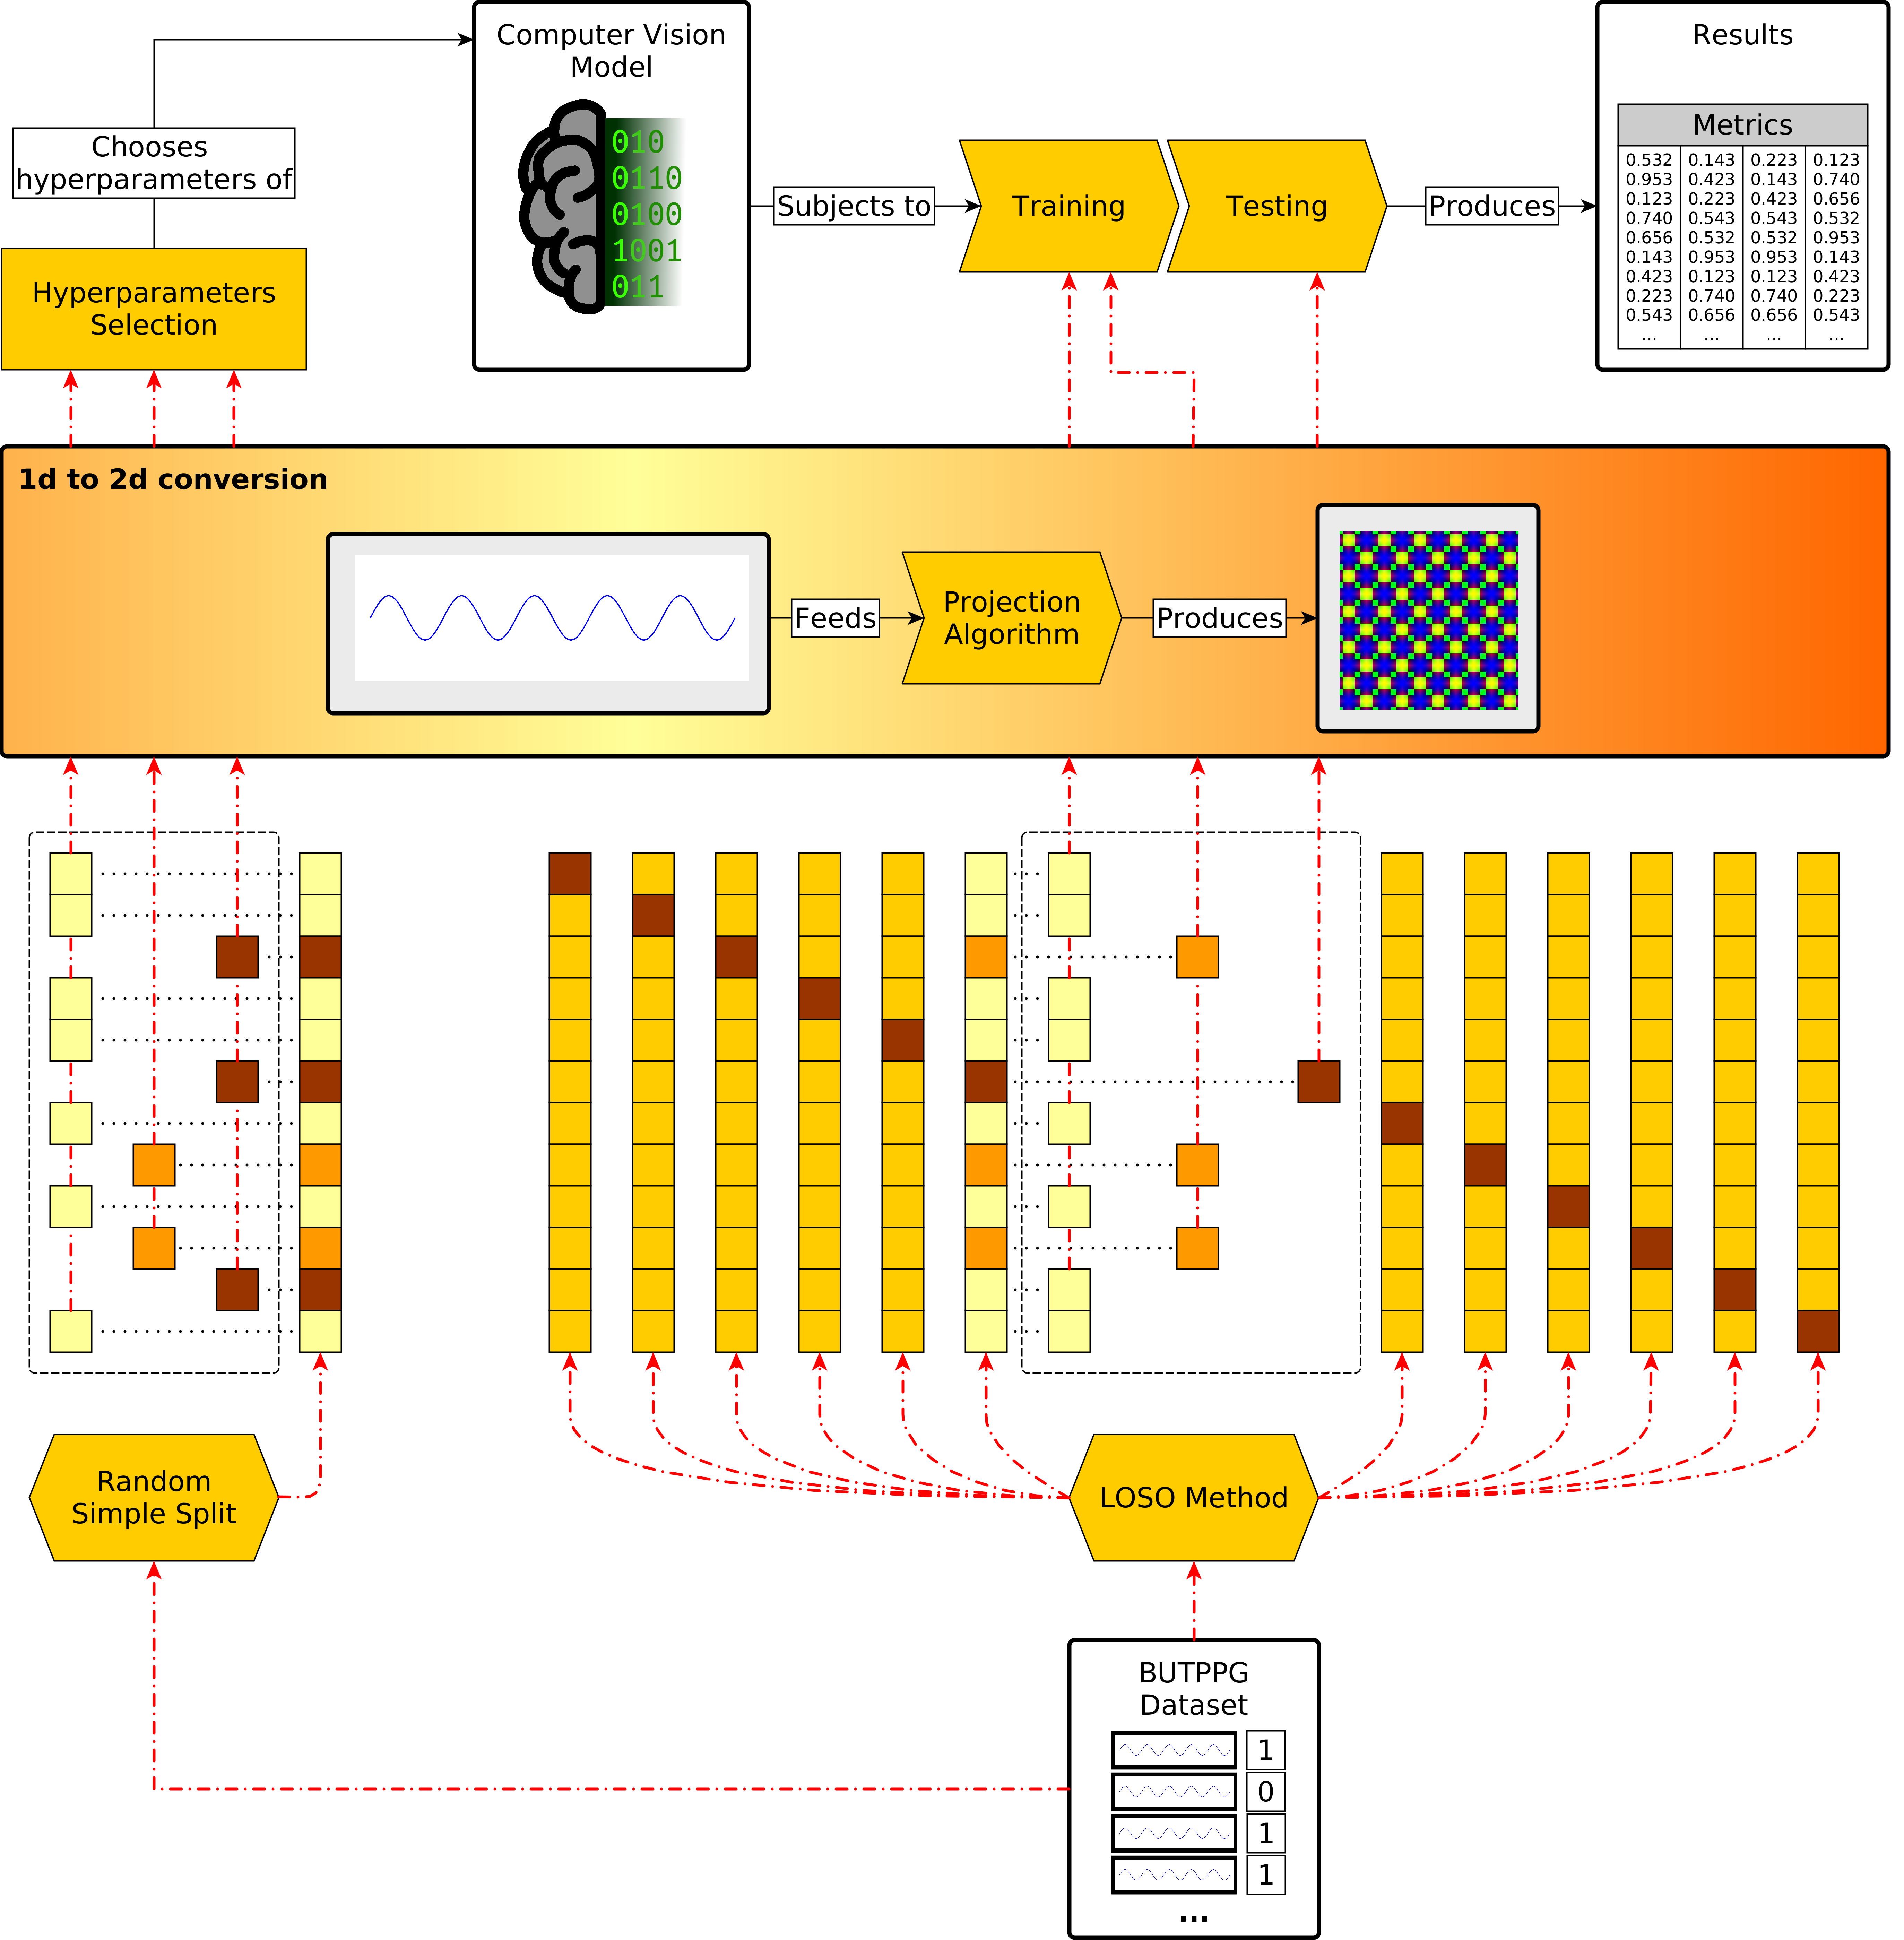
\includegraphics[width=\textwidth]{img/framework.png}
	\caption{The framework of the experiment. Red dotted arrows indicates data flow that sources from the  BUTPPG Dataset, while the full black lines, labeled with an verb, represent a relationship ``A do B'', where the arrow starts on A and end on B. Notice that the figure presents the training-testing cycle for only one of the twelve folds. The above schema is replicated for each combination of  Computer Vision Model and Projection Algorithm.}
	\label{fig:framework}
\end{figure}


The Figure \ref{fig:framework} expresses how I did the experiment for the \gls{CV} models. A first observation is that the main difference from the framework applied to non-\gls{CV} models is that the 1d to 2d conversion acts as a frontier between the dataset and the rest of the components. That means the non-\gls{CV} models experiment can be expressed using almost the same schema by removing that conversion block. With that, the experiment began by the Hyperparameters Selecion, splitting the \gls{BUTPPG} dataset using simple division for the purpose of, subsequentially, selecting the best hyperparameters of the \gls{CV}. With the best hyperparameters chosen, all models, including the non \gls{CV} models, will be evaluated using the \gls{LOSO} strategy. For each fold, I subjected the model to a training procedure that repeats epocs of training-and-validating until the early stopper interferes. Then, the model is tested, producing the metrics for that fold.

\subsection{The implementation details}

Presented the general concepts, in this section I discuss some details, following the practical sequence of events. I begin describing the process until the training. I done it by using the Python multithreading data feeding solution, named Data Loader\footnote{Documentation avaliable at \url{https://pytorch.org/docs/stable/data.html\#torch.utils.data.DataLoader}}. I configured it to load in batches of size 32. But, before loading the batches, I did the training dataset balancing using the Imbalanced Learn \cite{ImbalancedLearn} implementation of the random oversampling\footnote{Documentation avaliable at \url{https://imbalanced-learn.org/stable/references/generated/imblearn.over_sampling.RandomOverSampler.html\#imblearn.over_sampling.RandomOverSampler}}. Then, the batches are loaded transforming the signal into its images using the projection algorithm implementations of the PyTS Python library \cite{PyTS}. Even though the signals are now 2d, the width, height and number of channels dimensions are incompatible with the networks inputs. To solve this, I applyed the Pytorch resize transform\footnote{Documentation avaliable at \url{https://pytorch.org/vision/stable/generated/torchvision.transforms.Resize.html}} to ajust the width and the height; and, to ajust the model to the number of channels, I added an additional layer with 4 channels that I use in a pointwise convolution that outputs to the original model input layer, which contained 3 channels. For some models, I replaced the input layer with one containing the desired number of channels.

The \gls{CV} models were trained using a single NVIDIA RTX 3090 TI. For training, I used the Pytorch implementation of the Adam optmization algorithm\footnote{Documentation avaliable at \url{https://pytorch.org/docs/stable/generated/torch.optim.Adam.html\#torch.optim.Adam}}, which uses the gradients evaluated by the Pytorch autograd engine \cite{Pytorch}. The loss class (which, in our case, is the Cross Entropy Loss\footnote{Documentation avaliable at \url{https://pytorch.org/docs/stable/generated/torch.nn.CrossEntropyLoss.html\#torch.nn.CrossEntropyLoss}}) backpropagates the gradients based of the model foward pass errors. For the models testing, I used the Sklearn \cite{Sklearn} implementation of the metrics\footnote{Documentation at \url{https://scikit-learn.org/stable/modules/classes.html\#module-sklearn.metrics}}. For model memory measurement, I counted the summation of the size of each parameter and buffer tensors in the \gls{CV} models, while for the non-\gls{CV} models, I used the asizeof function\footnote{Documentation at \url{https://pympler.readthedocs.io/en/latest/library/asizeof.html}} of the Pympler library \cite{Pympler}. Finally, I descibe the inference time measurement, for which I extracted 500 measurement samples.  For the non-\gls{CV} models, I used the Python time method\footnote{Documentation at \url{https://docs.python.org/3/library/time.html\#time.time}}, of the time library, to measure instants of time. For the \gls{CV} models, I marked the time instants by using CUDA events interface provided by Pytorch\footnote{Documentation at \url{https://pytorch.org/docs/stable/generated/torch.cuda.Event.html}}, while, before measuring, performing 500 iterations to warm-up the GPU. 

\section{Experimental results}


In this section, I analyze the results will by comparing the metrics in the following order: firstly, I verify if the reescaled Cohen Kappa Score value is superior o equal to 90\%. Secondly, the F1-Score; and, lastly, the Precision score. Moreover, I considered the trade-off between models with respect to the memory consumption and the inference time, in that order. Since I considered a large set of models, I did the comparisions in sections. In each section, I consider one of the six before-presented computer vision model classifications: Transformers, Residual Nets, Mobile Oriented, Extreme Nets, Efficiency Oriented, and Diverse. In each of those sections, I selected the best combinatons of model variant and projection method, if at least one of them is sufficiently good. Subsequently, I will choose the best non-\gls{CV} models present in the Aeon toolkit. Lastly, I will determine the final best choices, also discussing the differences between the projection methods.

\subsection{Categories analysis}

\subsubsection{Transformers}

I tested four transformers the Vision Transformer, the Multi-axis Vision Transformer, the Shifted Windows Transformer and its second version. The Vision Transformer is the base model of the others. It transforms the visual input into into a word where the letters are linear embedings of subimages obtained by particioning the original image in a grid-like shape. Then, the other modules increments the original by using multiple layers and by changing the attention mechanisms. For instance, the MaxViT employs achitectural blocks where each alternates between two self-atention modes: grid attention, a mode of high granularity, and block attention, a mode of low granularity. The Swin Transformer, on the other hand, changes its attention in layer-level, by merging patches of the antecedent layer into a new one, and in block-level, by shifting the self-attention windows into different positions. Finally, the Swin Transformer V2 propose several specific improvements to the older version.

About the results, we can see on the tables \ref{tab:Averages_of_VisionTransformer}, \ref{tab:Averages_of_Maxvit}, \ref{tab:Averages_of_SwinTransformer}, and \ref{tab:Averages_of_SwinTransformer V2} that only the Swin Transformer V2 and the Vision Transformer variants obtained a Cohen Kappa score superior than 90\%. Specifically, for the Swin Transformer V2, only the standard variant combined with the \gls{Mix} method achieved such a score. For the Vision Transformer, only the large and base variants suprassed the limit. The variants with patch size $32\times 32$ did so by using the \gls{Mix}, while the variants with patch size $16 \times 16$ not only reached the score when combined with \gls{Mix} but also with \gls{RP}. Since both of the models reached a similar score, we observe the benchmarking metrics. We see in the Table \ref{tab:Memory_of_Transformers} that the Swin Transformer V2 S uses considerably less memory than the Vision Transformer. On the other hand, we observe in Figure \ref{fig:Time_of_Transformers} that the Swin Transformer V2 S have a slower inference speed if compared to the Vision Transformer variants. However, because I consider the memory consumption as a factor of major importance, I selected for this section the Swin Transformer V2 standard variant with \gls{Mix}.

\AveragesTable{Vision Transformer}{VisionTransformer}
\AveragesTable{MaxViT}{Maxvit}
\AveragesTable{Swin Transformer~V2}{SwinTransformer}
\AveragesTable{Swin Transformer~V2}{SwinTransformerV2}


\IncludeMemoryTable{Transformers}{Transformers}

\begin{figure}[h!]
	\includegraphics[width=\timePlotsWidth]{img/resultados/boxplots/benchmark_of_VisionTransformer.pdf}
	\includegraphics[width=\timePlotsWidth]{img/resultados/boxplots/benchmark_of_SwinTransformer.pdf}
	\includegraphics[width=\timePlotsWidth]{img/resultados/boxplots/benchmark_of_SwinTransformer V2.pdf}
	\includegraphics[width=\timePlotsWidth]{img/resultados/boxplots/benchmark_of_MaxVit.pdf}
	\caption{\TimePlotsDescription{Transformers}}
	\label{fig:Time_of_Transformers}
\end{figure}


\FloatBarrier

\subsubsection{Residual Nets}

This section analyzes the ResNet itself and its variations. The ResNet is a model that introduced the residual conections, links between non-adjacent layers that bypasses intermediate layers. As its variations, I analyzed two: the Wide ResNet and the ResNeXt. The first one widens the original net by increasing the number of channels per block, with the intention of providing an alternative to increasing the layer depth. The second one employs a multipath philosophy, agreggating the paths by an additive operation. As oposed to the antecedent, it avoids increasing the width and the depth of the network by providing an additional dimension to increase. 

Of those models, only the original ResNet and the Wide ResNet achieved a suficient Cohen Kappa score, as we can see in the tables \ref{tab:Averages_of_ResNet}, \ref{tab:Averages_of_ResNeXt} and \ref{tab:Averages_of_Wide ResNet}. From the ResNet variants, the ones with 50 and 101 layers reached that score. Solely the Wide ResNet with 101 layers and 2 convolutions per block sucessfully score above the limit. Those models variants got those scores by employing the \gls{Mix} projection method. Comparing these last variants, we conclude that the Wide ResNet 101-2 variant with the \gls{Mix} method obtained the best score, both for Cohen Kappa and F1 scores. However, that Wide ResNet posesses the largest memory occupation, according to the table \ref{tab:Memory_of_ResNet based}. It also spends the fourth higher inference time, as seen in the figure \ref{fig:Time_of_ResNet based}. Despite those disavantages, the Wide ResNet 101-2 variant with the \gls{Mix} was the choice of this section, because I prioritize the classification metrics over the benchmarking ones.

\AveragesTable{ResNet}{ResNet}
\AveragesTable{ResNeXt}{ResNeXt}
\AveragesTable{Wide ResNet}{WideResNet}



\IncludeMemoryTable{ResNet based}{Residual Nets}

\begin{figure}[h!]
	\includegraphics[width=\timePlotsWidth]{img/resultados/boxplots/benchmark_of_ResNet.pdf}
	\includegraphics[width=\timePlotsWidth]{img/resultados/boxplots/benchmark_of_Wide ResNet.pdf}
	\includegraphics[width=\timePlotsWidth]{img/resultados/boxplots/benchmark_of_ResNeXt.pdf}
	\caption{\TimePlotsDescription{Residual Nets}}
	\label{fig:Time_of_ResNet based}
\end{figure}


\FloatBarrier

\subsubsection{Mobile Oriented}

This section explores the mobile oriented networks, that is, networks designed specifically for mobile hardware constraints. I tested three models: the MNASNet, the Mobile Net V2 and the Mobile Net V3. In cronologial order, the Mobile Net V2 comes first. This newtork proposes several achitectural changes to use less memory while mantaining accuracy, with inverted residual blocks being one of them. This proposed alteration swaps places of the high-channeled and low-channeled layers, which causes the connection between layers with a lower ammount of channels, reducing the number of parameters in that block. After the antecedent, researchers introduced the MNASNet. Its name stands for Mobile Neural Architecture Search. It select blocks to fit in a predefined achitectural skeleton, optimizing the model performance on real-world mobile hardware. Finally, the Mobile Net V3 combined both approaches, while also made changes such as adding the NetAdapt \cite{NetAdapt} algorithm in the achitectural search.

In those set of models, only the MNASNet obtained a sufficient Cohen Kappa score, as visible in the tables \ref{tab:Averages_of_MNASNet}, \ref{tab:Averages_of_MobileNet V2} e \ref{tab:Averages_of_MobileNet V3}. Specifically, the MNASNet with depth multiplier of 1.0, being that multiplier related to the number of channels dimension. It achieved that score combined with the \gls{Mix} projection method method. According to the table \ref{tab:Memory_of_Mobile nets} and the figure \ref{fig:Time_of_Mobile nets}, all of those networks have very small memory size, with values inferior to 30 MB. They also have very fast inference time, with medians bellow to 20 ms. For those reasons and since it was the only net to achieve the minimum accuracy requirements, I chose the MNASNet 1.0 with \gls{Mix}. 

\AveragesTable{MNASNet}{MNASNet}
\AveragesTable{MobileNet~V2}{MobileNetV2}
\AveragesTable{MobileNet~V3}{MobileNetV3}


\IncludeMemoryTable{Mobile nets}{Mobile Oriented}

\begin{figure}[h!]
	\includegraphics[width=\timePlotsWidth]{img/resultados/boxplots/benchmark_of_MobileNet V2.pdf}
	\includegraphics[width=\timePlotsWidth]{img/resultados/boxplots/benchmark_of_MobileNet V3.pdf}
	\includegraphics[width=\timePlotsWidth]{img/resultados/boxplots/benchmark_of_MNASNet.pdf}
	\caption{\TimePlotsDescription{Mobile Oriented}}
	\label{fig:Time_of_Mobile nets}
\end{figure}


\FloatBarrier

\subsubsection{Extreme Nets}

In this section, I discuss the results of neural models which focus on one concept and push it to the limit, such as the VGG, the DenseNet and the SqueezeNet. The VGG is a model that uses filters of size $3\times 3$ to allow adding more layers, increasing the depth model. On the other hand, the DenseNet applies skipping connections of the residual nets to all pairs of achitectural blocks present in the network, to achieve the benefits of having each layer closer to the input and the output of the model. Finally, the SqueezeNet tries to reach minimum memory usage not only by applying model compression techiniques but by introducing a new achitectural module which reduces the number of channels of a layer before another one with large convolutions filters, such as $3 \times 3$ filters. This reduces the number of parameters considerably.

Accordingly to the tables \ref{tab:Averages_of_DenseNet}, \ref{tab:Averages_of_VGG} and \ref{tab:Averages_of_AlexNet}, only the SqueezeNet and the VGG achieved the minimum Cohen Kappa score. For the Squeezenet, only the version 1.1, a more economic version if compared to the 1.0, reached the score, when combined to the \gls{RP} and the \gls{Mix}, with the \gls{Mix} giving the best score. The second was the VGG with 16 weight layers without batch normalization, when combined to the \gls{RP} projection method. Of those combinations, the SqueezeNet 1.1 with \gls{Mix} performed better than the others, while having less variance. Adding to that performance, the SqueezeNet 1.1 is the smalest model in memory, according to the table \ref{tab:Memory_of_Extreme models}. Furthermore, the SqueezeNets have low inference time if copared to the other models, as the Figure \ref{fig:Time_of_Extreme nets} depicts. Therefore, I selected for this section the SqueezeNet 1.1 with \gls{Mix}.

\begin{table}[h!]
	\adjustbox{width=\averagesTableWidth,center}{
		
\begin{tabular}[t]{lllll}
\toprule
Model & Projection & Cohen Kappa & F1 Score & Precision \\
\midrule
VGG: 11 & GAF & \textcolor[rgb]{0.5761353517,0.4238646483,0}{0.659} $\pm$ \textcolor[rgb]{0.9813763962,0.0186236038,0}{0.257} & \textcolor[rgb]{0.6130820399,0.3869179601,0}{0.840} $\pm$ \textcolor[rgb]{0.8179931192,0.1820068808,0}{0.182} & \textcolor[rgb]{0.5967365967,0.4032634033,0}{0.811} $\pm$ \textcolor[rgb]{0.6502693890,0.3497306110,0}{0.201} \\
 & MTF & \textcolor[rgb]{0.9501335708,0.0498664292,0}{0.500} $\pm$ \textcolor[rgb]{0.6654355176,0.3345644824,0}{0.174} & \textcolor[rgb]{0.8699186992,0.1300813008,0}{0.790} $\pm$ \textcolor[rgb]{0.4021860668,0.5000000000,0}{0.116} & \textcolor[rgb]{0.8974358974,0.1025641026,0}{0.729} $\pm$ \textcolor[rgb]{0.3672049968,0.5000000000,0}{0.155} \\
 & RP & \textcolor[rgb]{0.1763134461,0.5000000000,0}{0.829} $\pm$ \textcolor[rgb]{0.7355621391,0.2644378609,0}{0.192} & \textcolor[rgb]{0.5365853659,0.4634146341,0}{0.855} $\pm$ \textcolor[rgb]{0.8554220067,0.1445779933,0}{0.188} & \underline{\textcolor[rgb]{0.1025641026,0.5000000000,0}{0.944}} $\pm$ \textcolor[rgb]{0.2080512860,0.5000000000,0}{0.130} \\
 & Mix & \textcolor[rgb]{0.1665182547,0.5000000000,0}{0.833} $\pm$ \textcolor[rgb]{0.8482671723,0.1517328277,0}{0.222} & \underline{\textcolor[rgb]{0.1463414634,0.5000000000,0}{0.931}} $\pm$ \textcolor[rgb]{0.2240040057,0.5000000000,0}{0.087} & \underline{\textcolor[rgb]{0.2564102564,0.5000000000,0}{0.903}} $\pm$ \textcolor[rgb]{0.3075839781,0.5000000000,0}{0.146} \\
VGG: 11 BN & GAF & \textcolor[rgb]{0.8032056990,0.1967943010,0}{0.562} $\pm$ \textcolor[rgb]{0.5940200153,0.4059799847,0}{0.155} & \textcolor[rgb]{0.5691056911,0.4308943089,0}{0.848} $\pm$ \textcolor[rgb]{0.1349899397,0.5000000000,0}{0.073} & \textcolor[rgb]{0.7692307692,0.2307692308,0}{0.764} $\pm$ \textcolor[rgb]{0.2230100982,0.5000000000,0}{0.132} \\
 & MTF & \textcolor[rgb]{0.8432769368,0.1567230632,0}{0.545} $\pm$ \textcolor[rgb]{0.5762840628,0.4237159372,0}{0.151} & \textcolor[rgb]{0.5650406504,0.4349593496,0}{0.849} $\pm$ \textcolor[rgb]{0.3108773772,0.5000000000,0}{0.101} & \textcolor[rgb]{0.8205128205,0.1794871795,0}{0.750} $\pm$ \textcolor[rgb]{0.3384113914,0.5000000000,0}{0.151} \\
 & RP & \textcolor[rgb]{0.0685663402,0.5000000000,0}{0.875} $\pm$ \textcolor[rgb]{0.6443051694,0.3556948306,0}{0.169} & \underline{\textcolor[rgb]{0.1951219512,0.5000000000,0}{0.921}} $\pm$ \textcolor[rgb]{0.2928051170,0.5000000000,0}{0.098} & \underline{\textcolor[rgb]{0.1025641026,0.5000000000,0}{0.944}} $\pm$ \textcolor[rgb]{0.2080512860,0.5000000000,0}{0.130} \\
 & Mix & \textcolor[rgb]{0.1175422974,0.5000000000,0}{0.854} $\pm$ \textcolor[rgb]{0.7578007605,0.2421992395,0}{0.198} & \underline{\textcolor[rgb]{0.1707317073,0.5000000000,0}{0.926}} $\pm$ \textcolor[rgb]{0.2602523331,0.5000000000,0}{0.093} & \underline{\textcolor[rgb]{0.1794871795,0.5000000000,0}{0.924}} $\pm$ \textcolor[rgb]{0.2698456329,0.5000000000,0}{0.140} \\
VGG: 13 & GAF & \textcolor[rgb]{0.5583259127,0.4416740873,0}{0.667} $\pm$ \textcolor[rgb]{0.9341807785,0.0658192215,0}{0.244} & \textcolor[rgb]{0.4918699187,0.5000000000,0}{0.863} $\pm$ \textcolor[rgb]{0.4337722642,0.5000000000,0}{0.121} & \textcolor[rgb]{0.5641025641,0.4358974359,0}{0.819} $\pm$ \textcolor[rgb]{0.4793875881,0.5000000000,0}{0.173} \\
 & MTF & \textcolor[rgb]{0.9501335708,0.0498664292,0}{0.500} $\pm$ \textbf{\textcolor[rgb]{0.0000000000,0.5000000000,0}{0.000}} & \textcolor[rgb]{0.6260162602,0.3739837398,0}{0.837} $\pm$ \textcolor[rgb]{0.2377009274,0.5000000000,0}{0.090} & \textcolor[rgb]{0.8974358974,0.1025641026,0}{0.729} $\pm$ \textcolor[rgb]{0.2017357855,0.5000000000,0}{0.129} \\
 & RP & \textcolor[rgb]{0.0195903829,0.5000000000,0}{0.896} $\pm$ \textcolor[rgb]{0.7578007605,0.2421992395,0}{0.198} & \underline{\textcolor[rgb]{0.0813008130,0.5000000000,0}{0.944}} $\pm$ \textcolor[rgb]{0.3672244725,0.5000000000,0}{0.110} & \underline{\textcolor[rgb]{0.1538461538,0.5000000000,0}{0.931}} $\pm$ \textcolor[rgb]{0.4332280526,0.5000000000,0}{0.166} \\
 & Mix & \textcolor[rgb]{0.0685663402,0.5000000000,0}{0.875} $\pm$ \textcolor[rgb]{0.7623521573,0.2376478427,0}{0.199} & \underline{\textcolor[rgb]{0.0853658537,0.5000000000,0}{0.943}} $\pm$ \textcolor[rgb]{0.2161475738,0.5000000000,0}{0.086} & \underline{\textcolor[rgb]{0.1794871795,0.5000000000,0}{0.924}} $\pm$ \textcolor[rgb]{0.2698456329,0.5000000000,0}{0.140} \\
VGG: 13 BN & GAF & \textcolor[rgb]{0.9501335708,0.0498664292,0}{0.500} $\pm$ \textbf{\textcolor[rgb]{0.0000000000,0.5000000000,0}{0.000}} & \textcolor[rgb]{0.6260162602,0.3739837398,0}{0.837} $\pm$ \textcolor[rgb]{0.2377009274,0.5000000000,0}{0.090} & \textcolor[rgb]{0.8974358974,0.1025641026,0}{0.729} $\pm$ \textcolor[rgb]{0.2017357855,0.5000000000,0}{0.129} \\
 & MTF & \textcolor[rgb]{0.8788958148,0.1211041852,0}{0.530} $\pm$ \textcolor[rgb]{0.6254149914,0.3745850086,0}{0.164} & \textcolor[rgb]{0.6463414634,0.3536585366,0}{0.833} $\pm$ \textcolor[rgb]{0.3913485406,0.5000000000,0}{0.114} & \textcolor[rgb]{0.8461538462,0.1538461538,0}{0.743} $\pm$ \textcolor[rgb]{0.3502477607,0.5000000000,0}{0.153} \\
 & RP & \textcolor[rgb]{0.1665182547,0.5000000000,0}{0.833} $\pm$ \textcolor[rgb]{0.9410679338,0.0589320662,0}{0.246} & \underline{\textcolor[rgb]{0.1991869919,0.5000000000,0}{0.921}} $\pm$ \textcolor[rgb]{0.4957921792,0.5000000000,0}{0.131} & \textcolor[rgb]{0.2820512821,0.5000000000,0}{0.896} $\pm$ \textcolor[rgb]{0.6330964479,0.3669035521,0}{0.198} \\
 & Mix & \textcolor[rgb]{0.0739091719,0.5000000000,0}{0.873} $\pm$ \textcolor[rgb]{0.7220818610,0.2779181390,0}{0.189} & \underline{\textcolor[rgb]{0.2378048780,0.5000000000,0}{0.913}} $\pm$ \textcolor[rgb]{0.6415115340,0.3584884660,0}{0.154} & \underline{\textcolor[rgb]{0.1794871795,0.5000000000,0}{0.924}} $\pm$ \textcolor[rgb]{0.2698456329,0.5000000000,0}{0.140} \\
VGG: 16 & GAF & \textcolor[rgb]{0.7542297418,0.2457702582,0}{0.583} $\pm$ \textcolor[rgb]{0.6224579299,0.3775420701,0}{0.163} & \textcolor[rgb]{0.5110864745,0.4889135255,0}{0.860} $\pm$ \textbf{\textcolor[rgb]{0.0000000000,0.5000000000,0}{0.052}} & \textcolor[rgb]{0.7086247086,0.2913752914,0}{0.780} $\pm$ \textcolor[rgb]{0.1071119150,0.5000000000,0}{0.113} \\
 & MTF & \textcolor[rgb]{0.9501335708,0.0498664292,0}{0.500} $\pm$ \textbf{\textcolor[rgb]{0.0000000000,0.5000000000,0}{0.000}} & \textcolor[rgb]{0.6260162602,0.3739837398,0}{0.837} $\pm$ \textcolor[rgb]{0.2377009274,0.5000000000,0}{0.090} & \textcolor[rgb]{0.8974358974,0.1025641026,0}{0.729} $\pm$ \textcolor[rgb]{0.2017357855,0.5000000000,0}{0.129} \\
 & RP & \underline{\textbf{\textcolor[rgb]{0.0000000000,0.5000000000,0}{0.904}}} $\pm$ \textcolor[rgb]{0.6937384685,0.3062615315,0}{0.181} & \underline{\textcolor[rgb]{0.1524390244,0.5000000000,0}{0.930}} $\pm$ \textcolor[rgb]{0.6254081161,0.3745918839,0}{0.151} & \underline{\textbf{\textcolor[rgb]{0.0000000000,0.5000000000,0}{0.972}}} $\pm$ \textbf{\textcolor[rgb]{0.0000000000,0.5000000000,0}{0.096}} \\
 & Mix & \textcolor[rgb]{0.0685663402,0.5000000000,0}{0.875} $\pm$ \textcolor[rgb]{0.7623521573,0.2376478427,0}{0.199} & \underline{\textcolor[rgb]{0.0853658537,0.5000000000,0}{0.943}} $\pm$ \textcolor[rgb]{0.2161475738,0.5000000000,0}{0.086} & \underline{\textcolor[rgb]{0.1794871795,0.5000000000,0}{0.924}} $\pm$ \textcolor[rgb]{0.2698456329,0.5000000000,0}{0.140} \\
VGG: 16 BN & GAF & \textcolor[rgb]{0.8539626002,0.1460373998,0}{0.541} $\pm$ \textcolor[rgb]{0.7491692816,0.2508307184,0}{0.196} & \textcolor[rgb]{0.5066518847,0.4933481153,0}{0.861} $\pm$ \textcolor[rgb]{0.2377250888,0.5000000000,0}{0.090} & \textcolor[rgb]{1.0000000000,0.0000000000,0}{0.701} $\pm$ \textcolor[rgb]{1.0000000000,0.0000000000,0}{0.257} \\
 & MTF & \textcolor[rgb]{0.7868803799,0.2131196201,0}{0.569} $\pm$ \textcolor[rgb]{0.6768896378,0.3231103622,0}{0.177} & \textcolor[rgb]{0.6747967480,0.3252032520,0}{0.828} $\pm$ \textcolor[rgb]{0.2405929417,0.5000000000,0}{0.090} & \textcolor[rgb]{0.7179487179,0.2820512821,0}{0.778} $\pm$ \textcolor[rgb]{0.3470343755,0.5000000000,0}{0.152} \\
 & RP & \textcolor[rgb]{0.6562778272,0.3437221728,0}{0.625} $\pm$ \textcolor[rgb]{0.7623521573,0.2376478427,0}{0.199} & \textcolor[rgb]{0.5325203252,0.4674796748,0}{0.856} $\pm$ \textcolor[rgb]{0.2226403475,0.5000000000,0}{0.087} & \textcolor[rgb]{0.6410256410,0.3589743590,0}{0.799} $\pm$ \textcolor[rgb]{0.1811818997,0.5000000000,0}{0.125} \\
 & Mix & \textcolor[rgb]{0.0195903829,0.5000000000,0}{0.896} $\pm$ \textcolor[rgb]{0.7578007605,0.2421992395,0}{0.198} & \underline{\textbf{\textcolor[rgb]{0.0000000000,0.5000000000,0}{0.960}}} $\pm$ \textcolor[rgb]{0.1431882304,0.5000000000,0}{0.075} & \underline{\textcolor[rgb]{0.0769230769,0.5000000000,0}{0.951}} $\pm$ \textcolor[rgb]{0.1159746586,0.5000000000,0}{0.115} \\
VGG: 19 & GAF & \textcolor[rgb]{0.7898486198,0.2101513802,0}{0.568} $\pm$ \textcolor[rgb]{0.4463877156,0.5000000000,0}{0.117} & \textcolor[rgb]{0.5365853659,0.4634146341,0}{0.855} $\pm$ \textcolor[rgb]{0.0032158844,0.5000000000,0}{0.052} & \textcolor[rgb]{0.7179487179,0.2820512821,0}{0.778} $\pm$ \textcolor[rgb]{0.0765276710,0.5000000000,0}{0.109} \\
 & MTF & \textcolor[rgb]{1.0000000000,0.0000000000,0}{0.479} $\pm$ \textcolor[rgb]{0.2975918104,0.5000000000,0}{0.078} & \textcolor[rgb]{0.9410569106,0.0589430894,0}{0.776} $\pm$ \textcolor[rgb]{0.5514159208,0.4485840792,0}{0.139} & \textcolor[rgb]{0.8717948718,0.1282051282,0}{0.736} $\pm$ \textcolor[rgb]{0.3598231789,0.5000000000,0}{0.154} \\
 & RP & \textcolor[rgb]{0.1175422974,0.5000000000,0}{0.854} $\pm$ \textcolor[rgb]{0.8604148146,0.1395851854,0}{0.225} & \underline{\textcolor[rgb]{0.1422764228,0.5000000000,0}{0.932}} $\pm$ \textcolor[rgb]{0.3739711043,0.5000000000,0}{0.111} & \underline{\textcolor[rgb]{0.2307692308,0.5000000000,0}{0.910}} $\pm$ \textcolor[rgb]{0.4708846452,0.5000000000,0}{0.172} \\
 & Mix & \textcolor[rgb]{0.5093499555,0.4906500445,0}{0.688} $\pm$ \textcolor[rgb]{0.8276249752,0.1723750248,0}{0.217} & \textcolor[rgb]{0.4146341463,0.5000000000,0}{0.879} $\pm$ \textcolor[rgb]{0.1596186962,0.5000000000,0}{0.077} & \textcolor[rgb]{0.4871794872,0.5000000000,0}{0.840} $\pm$ \textcolor[rgb]{0.2974495959,0.5000000000,0}{0.144} \\
VGG: 19 BN & GAF & \textcolor[rgb]{0.8358563372,0.1641436628,0}{0.549} $\pm$ \textcolor[rgb]{0.7618477893,0.2381522107,0}{0.199} & \textcolor[rgb]{0.8699186992,0.1300813008,0}{0.790} $\pm$ \textcolor[rgb]{0.6304392736,0.3695607264,0}{0.152} & \textcolor[rgb]{0.7948717949,0.2051282051,0}{0.757} $\pm$ \textcolor[rgb]{0.4708846452,0.5000000000,0}{0.172} \\
 & MTF & \textcolor[rgb]{0.8254674978,0.1745325022,0}{0.553} $\pm$ \textcolor[rgb]{1.0000000000,0.0000000000,0}{0.262} & \textcolor[rgb]{1.0000000000,0.0000000000,0}{0.764} $\pm$ \textcolor[rgb]{1.0000000000,0.0000000000,0}{0.211} & \textcolor[rgb]{0.8461538462,0.1538461538,0}{0.743} $\pm$ \textcolor[rgb]{0.7343347100,0.2656652900,0}{0.215} \\
 & RP & \textcolor[rgb]{0.0685663402,0.5000000000,0}{0.875} $\pm$ \textcolor[rgb]{0.7623521573,0.2376478427,0}{0.199} & \underline{\textcolor[rgb]{0.1666666667,0.5000000000,0}{0.927}} $\pm$ \textcolor[rgb]{0.4030274280,0.5000000000,0}{0.116} & \underline{\textcolor[rgb]{0.1538461538,0.5000000000,0}{0.931}} $\pm$ \textcolor[rgb]{0.4332280526,0.5000000000,0}{0.166} \\
 & Mix & \textcolor[rgb]{0.4603739982,0.5000000000,0}{0.708} $\pm$ \textcolor[rgb]{0.9841924031,0.0158075969,0}{0.257} & \textcolor[rgb]{0.3821138211,0.5000000000,0}{0.885} $\pm$ \textcolor[rgb]{0.4457804883,0.5000000000,0}{0.123} & \textcolor[rgb]{0.5128205128,0.4871794872,0}{0.833} $\pm$ \textcolor[rgb]{0.6106582296,0.3893417704,0}{0.195} \\
\bottomrule
\end{tabular}


	}
	\caption{}
\end{table}

\begin{table}[h!]
	\adjustbox{width=\averagesTableWidth,center}{
		
\begin{tabular}{lllll}
\toprule
Model & Projection & Cohen Kappa & F1 Score & Precision \\
\midrule
DenseNet: 121 & GAF & \textcolor[rgb]{0.6608933455,0.3391066545,0}{0.621} $\pm$ \textcolor[rgb]{0.9041130657,0.0958869343,0}{0.248} & \textcolor[rgb]{0.6082844097,0.3917155903,0}{0.795} $\pm$ \textcolor[rgb]{0.8643144405,0.1356855595,0}{0.190} & \textcolor[rgb]{0.6744186047,0.3255813953,0}{0.799} $\pm$ \textcolor[rgb]{0.5590408937,0.4409591063,0}{0.196} \\
 & MTF & \textcolor[rgb]{0.9525979945,0.0474020055,0}{0.500} $\pm$ \textbf{\textcolor[rgb]{0.0000000000,0.5000000000,0}{0.000}} & \textcolor[rgb]{0.4337899543,0.5000000000,0}{0.837} $\pm$ \textcolor[rgb]{0.2073760791,0.5000000000,0}{0.090} & \textcolor[rgb]{0.9069767442,0.0930232558,0}{0.729} $\pm$ \textcolor[rgb]{0.3669781154,0.5000000000,0}{0.129} \\
 & RP & \textcolor[rgb]{0.3008204193,0.5000000000,0}{0.771} $\pm$ \textcolor[rgb]{0.8198234888,0.1801765112,0}{0.225} & \underline{\textcolor[rgb]{0.1043705153,0.5000000000,0}{0.917}} $\pm$ \textcolor[rgb]{0.2718715508,0.5000000000,0}{0.099} & \underline{\textbf{\textcolor[rgb]{0.0000000000,0.5000000000,0}{1.000}}} $\pm$ \textbf{\textcolor[rgb]{0.0000000000,0.5000000000,0}{0.000}} \\
 & Mix & \textcolor[rgb]{0.0802187785,0.5000000000,0}{0.862} $\pm$ \textcolor[rgb]{0.7731356242,0.2268643758,0}{0.212} & \underline{\textcolor[rgb]{0.1679712981,0.5000000000,0}{0.902}} $\pm$ \textcolor[rgb]{0.7127121360,0.2872878640,0}{0.167} & \underline{\textcolor[rgb]{0.2325581395,0.5000000000,0}{0.931}} $\pm$ \textcolor[rgb]{0.4733152883,0.5000000000,0}{0.166} \\
DenseNet: 161 & GAF & \textcolor[rgb]{0.8155575813,0.1844424187,0}{0.557} $\pm$ \textcolor[rgb]{0.6127939876,0.3872060124,0}{0.168} & \textcolor[rgb]{0.9001956947,0.0998043053,0}{0.724} $\pm$ \textcolor[rgb]{0.8705294077,0.1294705923,0}{0.191} & \textcolor[rgb]{0.7103594080,0.2896405920,0}{0.788} $\pm$ \textcolor[rgb]{0.5454934107,0.4545065893,0}{0.191} \\
 & MTF & \textcolor[rgb]{0.5296262534,0.4703737466,0}{0.676} $\pm$ \textcolor[rgb]{0.8718566415,0.1281433585,0}{0.239} & \textcolor[rgb]{0.5136986301,0.4863013699,0}{0.818} $\pm$ \textcolor[rgb]{0.7123620115,0.2876379885,0}{0.167} & \textcolor[rgb]{0.5116279070,0.4883720930,0}{0.847} $\pm$ \textcolor[rgb]{0.5804275230,0.4195724770,0}{0.204} \\
 & RP & \textbf{\textcolor[rgb]{0.0000000000,0.5000000000,0}{0.896}} $\pm$ \textcolor[rgb]{0.6087717266,0.3912282734,0}{0.167} & \underline{\textcolor[rgb]{0.0195694716,0.5000000000,0}{0.938}} $\pm$ \textcolor[rgb]{0.2275213798,0.5000000000,0}{0.093} & \underline{\textcolor[rgb]{0.1860465116,0.5000000000,0}{0.944}} $\pm$ \textcolor[rgb]{0.3698791733,0.5000000000,0}{0.130} \\
 & Mix & \textcolor[rgb]{0.3509571559,0.5000000000,0}{0.750} $\pm$ \textcolor[rgb]{0.8681986203,0.1318013797,0}{0.238} & \underline{\textcolor[rgb]{0.1467710372,0.5000000000,0}{0.907}} $\pm$ \textcolor[rgb]{0.1743396851,0.5000000000,0}{0.085} & \textcolor[rgb]{0.4651162791,0.5000000000,0}{0.861} $\pm$ \textcolor[rgb]{0.4217271436,0.5000000000,0}{0.148} \\
DenseNet: 169 & GAF & \textcolor[rgb]{1.0000000000,0.0000000000,0}{0.480} $\pm$ \textcolor[rgb]{0.3750153542,0.5000000000,0}{0.103} & \textcolor[rgb]{1.0000000000,0.0000000000,0}{0.700} $\pm$ \textcolor[rgb]{1.0000000000,0.0000000000,0}{0.211} & \textcolor[rgb]{0.7813953488,0.2186046512,0}{0.767} $\pm$ \textcolor[rgb]{0.5347281177,0.4652718823,0}{0.188} \\
 & MTF & \textcolor[rgb]{0.5849285931,0.4150714069,0}{0.653} $\pm$ \textcolor[rgb]{0.9495951119,0.0504048881,0}{0.261} & \textcolor[rgb]{0.3522504892,0.5000000000,0}{0.857} $\pm$ \textcolor[rgb]{0.4821490246,0.5000000000,0}{0.132} & \textcolor[rgb]{0.6511627907,0.3488372093,0}{0.806} $\pm$ \textcolor[rgb]{0.5486194730,0.4513805270,0}{0.192} \\
 & RP & \textcolor[rgb]{0.6244302644,0.3755697356,0}{0.636} $\pm$ \textcolor[rgb]{1.0000000000,0.0000000000,0}{0.275} & \textcolor[rgb]{0.3913894325,0.5000000000,0}{0.848} $\pm$ \textcolor[rgb]{0.4943543354,0.5000000000,0}{0.133} & \textcolor[rgb]{0.6744186047,0.3255813953,0}{0.799} $\pm$ \textcolor[rgb]{0.4351978611,0.5000000000,0}{0.153} \\
 & Mix & \textcolor[rgb]{0.1504102097,0.5000000000,0}{0.833} $\pm$ \textcolor[rgb]{0.8082489293,0.1917510707,0}{0.222} & \underline{\textcolor[rgb]{0.0213485145,0.5000000000,0}{0.938}} $\pm$ \textcolor[rgb]{0.1994619916,0.5000000000,0}{0.088} & \underline{\textcolor[rgb]{0.2790697674,0.5000000000,0}{0.917}} $\pm$ \textcolor[rgb]{0.4114646048,0.5000000000,0}{0.144} \\
DenseNet: 201 & GAF & \textcolor[rgb]{0.7119416591,0.2880583409,0}{0.600} $\pm$ \textcolor[rgb]{0.9318485438,0.0681514562,0}{0.256} & \textcolor[rgb]{0.3344600605,0.5000000000,0}{0.861} $\pm$ \textcolor[rgb]{0.3774431799,0.5000000000,0}{0.116} & \textcolor[rgb]{0.9069767442,0.0930232558,0}{0.729} $\pm$ \textcolor[rgb]{0.8299131753,0.1700868247,0}{0.291} \\
 & MTF & \textcolor[rgb]{0.8122151322,0.1877848678,0}{0.558} $\pm$ \textcolor[rgb]{0.8138252624,0.1861747376,0}{0.223} & \textcolor[rgb]{0.3639921722,0.5000000000,0}{0.854} $\pm$ \textbf{\textcolor[rgb]{0.0000000000,0.5000000000,0}{0.058}} & \textcolor[rgb]{1.0000000000,0.0000000000,0}{0.701} $\pm$ \textcolor[rgb]{1.0000000000,0.0000000000,0}{0.351} \\
 & RP & \textcolor[rgb]{0.5113947129,0.4886052871,0}{0.683} $\pm$ \textcolor[rgb]{0.6649895152,0.3350104848,0}{0.183} & \textcolor[rgb]{0.6996086106,0.3003913894,0}{0.773} $\pm$ \textcolor[rgb]{0.7894014871,0.2105985129,0}{0.179} & \textcolor[rgb]{0.3720930233,0.5000000000,0}{0.889} $\pm$ \textcolor[rgb]{0.4996792473,0.5000000000,0}{0.175} \\
 & Mix & \textcolor[rgb]{0.0501367366,0.5000000000,0}{0.875} $\pm$ \textcolor[rgb]{0.7263870807,0.2736129193,0}{0.199} & \underline{\textbf{\textcolor[rgb]{0.0000000000,0.5000000000,0}{0.943}}} $\pm$ \textcolor[rgb]{0.1850021874,0.5000000000,0}{0.086} & \underline{\textcolor[rgb]{0.2558139535,0.5000000000,0}{0.924}} $\pm$ \textcolor[rgb]{0.3982647268,0.5000000000,0}{0.140} \\
\bottomrule
\end{tabular}


	}
	\caption{}
\end{table}


\IncludeMemoryTable{Extreme models}{Extreme Nets}

\begin{figure}[h!]
	\includegraphics[width=\timePlotsWidth]{img/resultados/boxplots/benchmark_of_VGG.pdf}
	\includegraphics[width=\timePlotsWidth]{img/resultados/boxplots/benchmark_of_DenseNet.pdf}
	\caption{\TimePlotsDescription{Extreme Nets}}
	\label{fig:Time_of_Extreme nets}
\end{figure}


\FloatBarrier

\subsubsection{Efficiency Oriented}

In this setion I discuss the models that researchers designed to efficiently utilize resources. For this work, I elaborate on the ShuffleNet V2, EfficientNet and EfficientNet V2. The first one is the ShuffleNet V2, sucessor of the ShuffleNet, which introduced the channel shuffle operator to allow information exchange among channels. It changes its predecessor by proposing, for each block, a channel split operation, to avoid costly operators such as grouped convolutions. Beside the shuffle nets, we have the efficient nets. The EfficientNet researchers studied the model scaling and created a compound resizing method that proportionally increase multiple dimensions, such as depth, number of channels and resolution. This allowed to create a very efficient base model that the researchers scaled up to bigger variants that mantain the advantages of the original. Finnaly, the EfficientNet V2 reformulated the antecessor by proposing a non-proportional scaling and by employing network architectural search. Additionally, it employed progressive learning by gradually increasing the dataset regularization.  

We observe in the tables \ref{tab:Averages_of_ShuffleNet V2}, \ref{tab:Averages_of_EfficientNet}, and \ref{tab:Averages_of_EfficientNetV2} that none of the EfficientNet variants accomplished the minimum Cohen Kappa Score. Only a few variants of the other models remained. For the ShuffleNet V2, we see that the variants with $\times 1$ and $\times 0.5$ channels were the remainders, when combined with the \gls{Mix} method. For the EfficientNet V2, the unique variant that I tested, we observe that only the \gls{Mix} method allowed the minimum score. The scores that the ShuffleNet V2 variants reached are similar to the ones of the EfficientNet V2. However, the ShuffleNet V2 variants are smaller than the EfficientNet V2, as we can visualize in the Table \ref{tab:Memory_of_Efficiency Oriented}. Furthermore, the Figure \ref{fig:Time_of_Efficiency Oriented} shows that the ShuffleNet V2 variants are generally faster than the EfficientNet V2. For those reasons, I chose the smallest variant, ShuffleNet V2 $\times 0.5$, combined with the \gls{Mix} projection method. 

\AveragesTable{EfficientNet}{EfficientNet}
\AveragesTable{EfficientNet~V2}{EfficientNetV2}
\AveragesTable{ShuffleNet~V2}{ShuffleNetV2}


\begin{figure}[h!]
	\includegraphics[width=\timePlotsWidth]{img/resultados/boxplots/benchmark_of_EfficientNet.pdf}
	\includegraphics[width=\timePlotsWidth]{img/resultados/boxplots/benchmark_of_EfficientNetV2.pdf}
	\includegraphics[width=\timePlotsWidth]{img/resultados/boxplots/benchmark_of_ShuffleNet V2.pdf}
	\caption{\TimePlotsDescription{Efficiency-Oriented}}
	\label{fig:Time_of_Efficiency Oriented}
\end{figure}


\IncludeMemoryTable{Efficiency Oriented}{Efficiency Oriented}

\FloatBarrier


\subsubsection{Diverse}

In this section, I analyze the remaining models. They are: AlexNet, ConvNeXt and RegNet. Researchers introduced the first one in the old year of 2012. That net tested the idea of deep learning trained on multiple GPUs, allowing a faster training. Furthermore, it applyied dropout to reduce overfitting. In contrast, the ConvNeXt is a modern model of 2022, which reunites several convolutional techiniques of the past years, such as patchfied convolutions, inverted bottlenecks and grouped convolutions. The researchers proposed that model to push the state of traditional convolutional networks to the limit. Differently of the antecedents, the RegNet employs the ideia of designing network spaces rather than individual nets. Those populations are caracterized by the restriction of the parameter space to a linear function. This created populations of networks that are more apropriate for random achitectural search. In this manner, I am testing networks with big differences among them.

Amid those models, only the RegNet and the AlexNet passed the minimum Cohen Kappa test, as we can infer from the tables \ref{tab:Averages_of_AlexNet}, \ref{tab:Averages_of_ConvNeXt}, and \ref{tab:Averages_of_RegNet}. The AlexNet did so by applying the \gls{Mix} method for its only variant. The RegNet, on the other hand, has a plenty of variants, that originate from two network design spaces: X, the base space, and Y, which adds a squeeze-and-excitation operation after the blocks of X. From those variants, only the 3.2 GF (Giga FLOPs) and 800 MF (Mega FLOPs) variants of the X network space and only the 400 MF and 800 MF variants of the Y network space reached the score. Most of them did so by applying the \gls{Mix}, with only one exception: The RegNet Y 400 MF did by using the \gls{RP}. Since the variants of both models scored similarly, we observe the Figure \ref{fig:Time_of_Diverse} and the Table \ref{tab:Memory_of_Diverse}. The first observation is that the the AlexNet occupies, at least, two times more memory than most of the RegNet variants, including the ones with good score. The second one is that the AlexNet has faster inference speed than every model in this section. But, since the memory occupation is priority, I chose the RegNet over the AlexNet. Specifically, the RegNet Y 400 MF variant (with \gls{RP}), because it is the smallest.  

\begin{longtable}[t]{llllll}
\caption{All folds averages for each model in Diverse} \\
\toprule
Model & Projection & Accuracy & F1 Score & Precision & Recall \\
\midrule
\endfirsthead
\caption[]{All folds averages for each model in Diverse} \\
\toprule
Model & Projection & Accuracy & F1 Score & Precision & Recall \\
\midrule
\endhead
\midrule
\multicolumn{6}{r}{Continued on next page} \\
\midrule
\endfoot
\bottomrule
\endlastfoot
AlexNet & GAF & 0.750 $\pm$ 0.151 & 0.849 $\pm$ 0.101 & 0.750 $\pm$ 0.151 & \textbf{1.000 $\pm$ 0.000} \\
 & MTF & 0.708 $\pm$ 0.257 & 0.827 $\pm$ 0.174 & 0.773 $\pm$ 0.163 & 0.833 $\pm$ 0.333 \\
 & RP & 0.771 $\pm$ 0.167 & 0.819 $\pm$ 0.168 & 0.910 $\pm$ 0.135 & 0.812 $\pm$ 0.261 \\
 & Mix & \textbf{0.938 $\pm$ 0.113} & 0.955 $\pm$ 0.083 & 0.944 $\pm$ 0.130 & 0.979 $\pm$ 0.072 \\
ConvNeXt: Base & GAF & 0.688 $\pm$ 0.155 & 0.792 $\pm$ 0.137 & 0.764 $\pm$ 0.170 & 0.896 $\pm$ 0.211 \\
 & MTF & 0.625 $\pm$ 0.272 & 0.789 $\pm$ 0.159 & 0.667 $\pm$ 0.268 & 0.833 $\pm$ 0.333 \\
 & RP & 0.896 $\pm$ 0.167 & 0.913 $\pm$ 0.154 & 0.944 $\pm$ 0.130 & 0.924 $\pm$ 0.199 \\
 & Mix & 0.896 $\pm$ 0.129 & 0.926 $\pm$ 0.093 & 0.924 $\pm$ 0.140 & 0.951 $\pm$ 0.115 \\
ConvNeXt: Large & GAF & 0.750 $\pm$ 0.185 & 0.845 $\pm$ 0.124 & 0.785 $\pm$ 0.183 & 0.951 $\pm$ 0.115 \\
 & MTF & 0.750 $\pm$ 0.151 & 0.849 $\pm$ 0.101 & 0.750 $\pm$ 0.151 & \textbf{1.000 $\pm$ 0.000} \\
 & RP & 0.875 $\pm$ 0.169 & 0.896 $\pm$ 0.154 & 0.944 $\pm$ 0.130 & 0.896 $\pm$ 0.211 \\
 & Mix & 0.875 $\pm$ 0.169 & 0.896 $\pm$ 0.154 & 0.944 $\pm$ 0.130 & 0.896 $\pm$ 0.211 \\
ConvNeXt: Small & GAF & 0.812 $\pm$ 0.188 & 0.885 $\pm$ 0.123 & 0.833 $\pm$ 0.195 & 0.979 $\pm$ 0.072 \\
 & MTF & 0.750 $\pm$ 0.185 & 0.845 $\pm$ 0.124 & 0.785 $\pm$ 0.183 & 0.951 $\pm$ 0.115 \\
 & RP & 0.896 $\pm$ 0.129 & 0.926 $\pm$ 0.093 & 0.924 $\pm$ 0.140 & 0.951 $\pm$ 0.115 \\
 & Mix & 0.917 $\pm$ 0.123 & 0.938 $\pm$ 0.093 & 0.944 $\pm$ 0.130 & 0.951 $\pm$ 0.115 \\
ConvNeXt: Tiny & GAF & 0.812 $\pm$ 0.155 & 0.884 $\pm$ 0.101 & 0.826 $\pm$ 0.168 & 0.979 $\pm$ 0.072 \\
 & MTF & 0.729 $\pm$ 0.129 & 0.833 $\pm$ 0.090 & 0.750 $\pm$ 0.151 & 0.972 $\pm$ 0.096 \\
 & RP & 0.854 $\pm$ 0.167 & 0.903 $\pm$ 0.113 & 0.875 $\pm$ 0.157 & 0.951 $\pm$ 0.115 \\
 & Mix & 0.875 $\pm$ 0.226 & 0.951 $\pm$ 0.086 & 0.939 $\pm$ 0.135 & 0.896 $\pm$ 0.291 \\
ShuffleNet V2: $\times$0.5 & GAF & 0.688 $\pm$ 0.241 & 0.784 $\pm$ 0.199 & 0.736 $\pm$ 0.210 & 0.875 $\pm$ 0.237 \\
 & MTF & 0.583 $\pm$ 0.289 & 0.851 $\pm$ 0.090 & 0.667 $\pm$ 0.280 & 0.667 $\pm$ 0.492 \\
 & RP & 0.854 $\pm$ 0.198 & 0.876 $\pm$ 0.190 & 0.910 $\pm$ 0.172 & 0.882 $\pm$ 0.232 \\
 & Mix & \textbf{0.938 $\pm$ 0.113} & 0.955 $\pm$ 0.083 & 0.944 $\pm$ 0.130 & 0.979 $\pm$ 0.072 \\
ShuffleNet V2: $\times$1.0 & GAF & 0.583 $\pm$ 0.268 & 0.744 $\pm$ 0.180 & 0.688 $\pm$ 0.285 & 0.764 $\pm$ 0.366 \\
 & MTF & 0.688 $\pm$ 0.264 & 0.862 $\pm$ 0.122 & 0.775 $\pm$ 0.184 & 0.833 $\pm$ 0.389 \\
 & RP & 0.688 $\pm$ 0.339 & 0.932 $\pm$ 0.095 & 0.885 $\pm$ 0.160 & 0.667 $\pm$ 0.492 \\
 & Mix & \textbf{0.938 $\pm$ 0.113} & 0.955 $\pm$ 0.083 & 0.944 $\pm$ 0.130 & 0.979 $\pm$ 0.072 \\
ShuffleNet V2: $\times$1.5 & GAF & 0.729 $\pm$ 0.129 & 0.837 $\pm$ 0.090 & 0.729 $\pm$ 0.129 & \textbf{1.000 $\pm$ 0.000} \\
 & MTF & 0.562 $\pm$ 0.285 & 0.772 $\pm$ 0.122 & 0.659 $\pm$ 0.248 & 0.708 $\pm$ 0.377 \\
 & RP & 0.604 $\pm$ 0.291 & 0.792 $\pm$ 0.207 & 0.767 $\pm$ 0.301 & 0.632 $\pm$ 0.465 \\
 & Mix & 0.833 $\pm$ 0.163 & 0.868 $\pm$ 0.148 & 0.951 $\pm$ 0.115 & 0.840 $\pm$ 0.220 \\
ShuffleNet V2: $\times$2.0 & GAF & 0.771 $\pm$ 0.167 & 0.861 $\pm$ 0.110 & 0.792 $\pm$ 0.179 & 0.979 $\pm$ 0.072 \\
 & MTF & 0.625 $\pm$ 0.250 & 0.700 $\pm$ 0.230 & 0.778 $\pm$ 0.234 & 0.736 $\pm$ 0.329 \\
 & RP & 0.562 $\pm$ 0.322 & 0.789 $\pm$ 0.189 & 0.629 $\pm$ 0.358 & 0.639 $\pm$ 0.437 \\
 & Mix & 0.833 $\pm$ 0.163 & 0.896 $\pm$ 0.106 & 0.847 $\pm$ 0.173 & 0.979 $\pm$ 0.072 \\
SqueezeNet: 1.0 & GAF & 0.729 $\pm$ 0.225 & 0.804 $\pm$ 0.192 & 0.771 $\pm$ 0.198 & 0.875 $\pm$ 0.237 \\
 & MTF & 0.667 $\pm$ 0.222 & 0.742 $\pm$ 0.197 & 0.812 $\pm$ 0.217 & 0.778 $\pm$ 0.296 \\
 & RP & 0.792 $\pm$ 0.209 & 0.816 $\pm$ 0.194 & 0.958 $\pm$ 0.144 & 0.771 $\pm$ 0.269 \\
 & Mix & 0.750 $\pm$ 0.282 & 0.838 $\pm$ 0.210 & 0.856 $\pm$ 0.211 & 0.771 $\pm$ 0.335 \\
SqueezeNet: 1.1 & GAF & 0.604 $\pm$ 0.249 & 0.819 $\pm$ 0.080 & 0.700 $\pm$ 0.105 & 0.833 $\pm$ 0.389 \\
 & MTF & 0.625 $\pm$ 0.272 & 0.794 $\pm$ 0.161 & 0.646 $\pm$ 0.249 & 0.861 $\pm$ 0.332 \\
 & RP & 0.896 $\pm$ 0.198 & 0.914 $\pm$ 0.168 & \textbf{0.972 $\pm$ 0.096} & 0.903 $\pm$ 0.230 \\
 & Mix & \textbf{0.938 $\pm$ 0.113} & 0.955 $\pm$ 0.083 & 0.944 $\pm$ 0.130 & 0.979 $\pm$ 0.072 \\
VGG: 11 & GAF & 0.729 $\pm$ 0.271 & 0.840 $\pm$ 0.182 & 0.811 $\pm$ 0.201 & 0.833 $\pm$ 0.333 \\
 & MTF & 0.667 $\pm$ 0.163 & 0.790 $\pm$ 0.116 & 0.729 $\pm$ 0.155 & 0.896 $\pm$ 0.155 \\
 & RP & 0.833 $\pm$ 0.195 & 0.855 $\pm$ 0.188 & 0.944 $\pm$ 0.130 & 0.840 $\pm$ 0.262 \\
 & Mix & 0.896 $\pm$ 0.129 & 0.931 $\pm$ 0.087 & 0.903 $\pm$ 0.146 & 0.979 $\pm$ 0.072 \\
VGG: 11 BN & GAF & 0.750 $\pm$ 0.107 & 0.848 $\pm$ 0.073 & 0.764 $\pm$ 0.132 & 0.979 $\pm$ 0.072 \\
 & MTF & 0.750 $\pm$ 0.151 & 0.849 $\pm$ 0.101 & 0.750 $\pm$ 0.151 & \textbf{1.000 $\pm$ 0.000} \\
 & RP & 0.896 $\pm$ 0.129 & 0.921 $\pm$ 0.098 & 0.944 $\pm$ 0.130 & 0.924 $\pm$ 0.140 \\
 & Mix & 0.896 $\pm$ 0.129 & 0.926 $\pm$ 0.093 & 0.924 $\pm$ 0.140 & 0.951 $\pm$ 0.115 \\
VGG: 13 & GAF & 0.792 $\pm$ 0.179 & 0.863 $\pm$ 0.121 & 0.819 $\pm$ 0.173 & 0.944 $\pm$ 0.130 \\
 & MTF & 0.729 $\pm$ 0.129 & 0.837 $\pm$ 0.090 & 0.729 $\pm$ 0.129 & \textbf{1.000 $\pm$ 0.000} \\
 & RP & 0.917 $\pm$ 0.163 & 0.944 $\pm$ 0.110 & 0.931 $\pm$ 0.166 & 0.979 $\pm$ 0.072 \\
 & Mix & 0.917 $\pm$ 0.123 & 0.943 $\pm$ 0.086 & 0.924 $\pm$ 0.140 & 0.979 $\pm$ 0.072 \\
VGG: 13 BN & GAF & 0.729 $\pm$ 0.129 & 0.837 $\pm$ 0.090 & 0.729 $\pm$ 0.129 & \textbf{1.000 $\pm$ 0.000} \\
 & MTF & 0.729 $\pm$ 0.167 & 0.833 $\pm$ 0.114 & 0.743 $\pm$ 0.153 & 0.972 $\pm$ 0.096 \\
 & RP & 0.875 $\pm$ 0.199 & 0.921 $\pm$ 0.131 & 0.896 $\pm$ 0.198 & 0.979 $\pm$ 0.072 \\
 & Mix & 0.896 $\pm$ 0.167 & 0.913 $\pm$ 0.154 & 0.924 $\pm$ 0.140 & 0.944 $\pm$ 0.192 \\
VGG: 16 & GAF & 0.729 $\pm$ 0.167 & 0.860 $\pm$ 0.052 & 0.780 $\pm$ 0.113 & 0.896 $\pm$ 0.291 \\
 & MTF & 0.729 $\pm$ 0.129 & 0.837 $\pm$ 0.090 & 0.729 $\pm$ 0.129 & \textbf{1.000 $\pm$ 0.000} \\
 & RP & 0.917 $\pm$ 0.163 & 0.930 $\pm$ 0.151 & \textbf{0.972 $\pm$ 0.096} & 0.924 $\pm$ 0.199 \\
 & Mix & 0.917 $\pm$ 0.123 & 0.943 $\pm$ 0.086 & 0.924 $\pm$ 0.140 & 0.979 $\pm$ 0.072 \\
VGG: 16 BN & GAF & 0.708 $\pm$ 0.257 & 0.861 $\pm$ 0.090 & 0.701 $\pm$ 0.257 & 0.917 $\pm$ 0.289 \\
 & MTF & 0.729 $\pm$ 0.129 & 0.828 $\pm$ 0.090 & 0.778 $\pm$ 0.152 & 0.924 $\pm$ 0.140 \\
 & RP & 0.771 $\pm$ 0.129 & 0.856 $\pm$ 0.087 & 0.799 $\pm$ 0.125 & 0.958 $\pm$ 0.144 \\
 & Mix & \textbf{0.938 $\pm$ 0.113} & \textbf{0.960 $\pm$ 0.075} & 0.951 $\pm$ 0.115 & 0.979 $\pm$ 0.072 \\
VGG: 19 & GAF & 0.771 $\pm$ 0.072 & 0.855 $\pm$ 0.052 & 0.778 $\pm$ 0.109 & 0.972 $\pm$ 0.096 \\
 & MTF & 0.667 $\pm$ 0.163 & 0.776 $\pm$ 0.139 & 0.736 $\pm$ 0.154 & 0.889 $\pm$ 0.217 \\
 & RP & 0.896 $\pm$ 0.167 & 0.932 $\pm$ 0.111 & 0.910 $\pm$ 0.172 & 0.979 $\pm$ 0.072 \\
 & Mix & 0.812 $\pm$ 0.113 & 0.879 $\pm$ 0.077 & 0.840 $\pm$ 0.144 & 0.951 $\pm$ 0.115 \\
VGG: 19 BN & GAF & 0.688 $\pm$ 0.188 & 0.790 $\pm$ 0.152 & 0.757 $\pm$ 0.172 & 0.868 $\pm$ 0.217 \\
 & MTF & 0.667 $\pm$ 0.268 & 0.764 $\pm$ 0.211 & 0.743 $\pm$ 0.215 & 0.833 $\pm$ 0.266 \\
 & RP & 0.896 $\pm$ 0.167 & 0.927 $\pm$ 0.116 & 0.931 $\pm$ 0.166 & 0.951 $\pm$ 0.115 \\
 & Mix & 0.812 $\pm$ 0.188 & 0.885 $\pm$ 0.123 & 0.833 $\pm$ 0.195 & 0.979 $\pm$ 0.072 \\
\end{longtable}


\begin{figure}[h!]
	\includegraphics[width=\timePlotsWidth]{img/resultados/boxplots/benchmark_of_AlexNet.pdf}
	\includegraphics[width=\timePlotsWidth]{img/resultados/boxplots/benchmark_of_ConvNeXt.pdf}
	\includegraphics[width=\timePlotsWidth]{img/resultados/boxplots/benchmark_of_RegNet.pdf}
	\caption{\TimePlotsDescription{Diverse}}
	\label{fig:Time_of_Diverse}
\end{figure}


\IncludeMemoryTable{Diverse}{Diverse}

\FloatBarrier

\subsection{Non-CV models comparison}

This section evaluate non-computationally-visual models, which I presented in the chapter \ref{Revisao_bibliografica}. Firstly, we observe in the Table \ref{tab:Averages_of_Non CV} that seven models achieved the minimum Cohen Kappa score. Among them only two achieved the greatest scores: the Random Interval Spectral Ensemble Classifier and the Temporal Dictionary Ensemble. But they got similar scores, so I refer to the Table \ref{tab:Memory_of_Non CV} and Figure \ref{fig:Time_of_Non CV} to decide which to choose. It is visible that the Random Interval Spectral Ensemble Classifier is faster in inference time than the Temporal Dictionary Ensemble, while the later is smaller in memory size. Due to the memory being a factor of major priority, I chose the Temporal Dictionary Ensemble. 	 

\AveragesTable{Non CV}


\IncludeMemoryTable{Non CV}{Non CV}

\begin{figure}[h!]
	\includegraphics[width=\timePlotsWidth]{img/resultados/boxplots/benchmark_of_Non CV.pdf}
	\caption{\TimePlotsDescription{Non-CV}}
	\label{fig:Time_of_Non CV}
\end{figure}


\FloatBarrier

\subsection{Best models comparison}

This section aggregates all choices that I made through all past sections. Observing their Table \ref{tab:Averages_of_Best Models}, we see that the two models obtained the best Cohen Kappa scores: the Temporal Dictionary Ensemble and the Wide ResNet 100-2 with \gls{Mix}, even though the other models obtained comparable score. That Wide ResNet obtained the highest Cohen Kappa score, but there are some considerations. Firstly, that model is the largest of this set, as we can read on table \ref{tab:Memory_of_Best Models}. Secondly, it did not obtained the best F1 score and Precision. Lastly, the Wide ResNet is the second slowest model as we can refer to the Figure \ref{fig:Time_of_Best Models}. On the other hand, the Temporal Dictionary Ensemble was the best in the usabiliy and security scores, F1-Score and Precision. It also is the fastest in inference and the smallest in memory. Therefore, I conclude that the \gls{CV} approach lead to a better accuracy, represented by the Wide ResNet 100-2 with \gls{Mix}, but the non-\gls{CV} approach can be more useful, since it uses less resources and is less inconvenient to the user.


\begin{table}[h!]
	\adjustbox{width=\averagesTableWidth,center}{
		
\begin{tabular}{lllll}
\toprule
Model & Projection & Cohen Kappa & F1 Score & Precision \\
\midrule
AlexNet & Mix & \underline{\textcolor[rgb]{0.7518796992,0.2481203008,0}{0.917}} $\pm$ \textcolor[rgb]{0.7679332798,0.2320667202,0}{0.163} & \underline{\textcolor[rgb]{0.4000000000,0.5000000000,0}{0.955}} $\pm$ \textcolor[rgb]{0.1825904218,0.5000000000,0}{0.083} & \underline{\textcolor[rgb]{1.0000000000,0.0000000000,0}{0.944}} $\pm$ \textcolor[rgb]{1.0000000000,0.0000000000,0}{0.130} \\
MNASNet: 1.0 & Mix & \underline{\textcolor[rgb]{0.7518796992,0.2481203008,0}{0.917}} $\pm$ \textcolor[rgb]{0.7679332798,0.2320667202,0}{0.163} & \underline{\textcolor[rgb]{0.4000000000,0.5000000000,0}{0.955}} $\pm$ \textcolor[rgb]{0.1825904218,0.5000000000,0}{0.083} & \underline{\textcolor[rgb]{1.0000000000,0.0000000000,0}{0.944}} $\pm$ \textcolor[rgb]{1.0000000000,0.0000000000,0}{0.130} \\
RandomIntervalSpectralEnsembleClassifier & Not projected & \underline{\textcolor[rgb]{0.3383458647,0.5000000000,0}{0.938}} $\pm$ \textcolor[rgb]{0.6753484915,0.3246515085,0}{0.155} & \underline{\textbf{\textcolor[rgb]{0.0000000000,0.5000000000,0}{0.971}}} $\pm$ \textbf{\textcolor[rgb]{0.0000000000,0.5000000000,0}{0.068}} & \underline{\textbf{\textcolor[rgb]{0.0000000000,0.5000000000,0}{0.972}}} $\pm$ \textbf{\textcolor[rgb]{0.0000000000,0.5000000000,0}{0.096}} \\
RegNet: Y; 400 MF & RP & \underline{\textcolor[rgb]{0.7518796992,0.2481203008,0}{0.917}} $\pm$ \textcolor[rgb]{0.7679332798,0.2320667202,0}{0.163} & \underline{\textcolor[rgb]{0.4000000000,0.5000000000,0}{0.955}} $\pm$ \textcolor[rgb]{0.1825904218,0.5000000000,0}{0.083} & \underline{\textcolor[rgb]{1.0000000000,0.0000000000,0}{0.944}} $\pm$ \textcolor[rgb]{1.0000000000,0.0000000000,0}{0.130} \\
SqueezeNet: 1.1 & Mix & \underline{\textcolor[rgb]{0.7518796992,0.2481203008,0}{0.917}} $\pm$ \textcolor[rgb]{0.7679332798,0.2320667202,0}{0.163} & \underline{\textcolor[rgb]{0.4000000000,0.5000000000,0}{0.955}} $\pm$ \textcolor[rgb]{0.1825904218,0.5000000000,0}{0.083} & \underline{\textcolor[rgb]{1.0000000000,0.0000000000,0}{0.944}} $\pm$ \textcolor[rgb]{1.0000000000,0.0000000000,0}{0.130} \\
VGG: 16 & RP & \underline{\textcolor[rgb]{1.0000000000,0.0000000000,0}{0.904}} $\pm$ \textcolor[rgb]{1.0000000000,0.0000000000,0}{0.181} & \underline{\textcolor[rgb]{1.0000000000,0.0000000000,0}{0.930}} $\pm$ \textcolor[rgb]{1.0000000000,0.0000000000,0}{0.151} & \underline{\textbf{\textcolor[rgb]{0.0000000000,0.5000000000,0}{0.972}}} $\pm$ \textbf{\textcolor[rgb]{0.0000000000,0.5000000000,0}{0.096}} \\
Vision Transformer: L 16 & RP & \underline{\textcolor[rgb]{0.7518796992,0.2481203008,0}{0.917}} $\pm$ \textcolor[rgb]{0.7679332798,0.2320667202,0}{0.163} & \underline{\textcolor[rgb]{0.4000000000,0.5000000000,0}{0.955}} $\pm$ \textcolor[rgb]{0.1825904218,0.5000000000,0}{0.083} & \underline{\textcolor[rgb]{1.0000000000,0.0000000000,0}{0.944}} $\pm$ \textcolor[rgb]{1.0000000000,0.0000000000,0}{0.130} \\
Wide ResNet: 101-2 & Mix & \underline{\textbf{\textcolor[rgb]{0.0000000000,0.5000000000,0}{0.955}}} $\pm$ \textbf{\textcolor[rgb]{0.0000000000,0.5000000000,0}{0.101}} & \underline{\textcolor[rgb]{0.1142857143,0.5000000000,0}{0.967}} $\pm$ \textcolor[rgb]{0.1202863916,0.5000000000,0}{0.078} & \underline{\textcolor[rgb]{1.0000000000,0.0000000000,0}{0.944}} $\pm$ \textcolor[rgb]{1.0000000000,0.0000000000,0}{0.130} \\
\bottomrule
\end{tabular}


	}
	\caption{\AveragesTableDescription{Best Models}}
	\label{tab:Averages_of_Best Models}
\end{table}


\IncludeMemoryTable{Best Models}{Best Models}

\begin{figure}[h!]
	\includegraphics[width=\timePlotsWidth]{img/resultados/boxplots/benchmark_of_Best Models.pdf}
	\caption{\TimePlotsDescription{best models}}
	\label{fig:Time_of_Best Models}
\end{figure}


\section{Limitations}

Even though the results are promising, we need to consider a series of limitations present in my experiment. One main observation is that I used only the BUTPPG dataset for testing. This has a series of implications in our context. Firstly, even though the proposed method allowed the use of \gls{CV} models with a good performance in the BUTPPG dataset, the same could not necessarily be concluded for different datasets. This is because different methods of measurement, sensor qualities, and signal lengths could lead to alterations on the obtained performance. Furthermore, the small size of the dataset resulted in a low ammount of testing, which makes the obtained results less trustable. A small dataset size also implies that the deep learning models had less resources to effectively learn. This contasts with the usual treatment for deep learning, where usually large ammounts of data feed the training of the model, allowing the proper adjustment of the large set of parameters. Therefore, my experiment would be more complete if I tested on different and larger datasets.

Other limit is that I did not explored all the options avaliable, in terms of models and hyperparameters. For instance, I did left out some of the models of the Pytorch and the Aeon libraries. Examples of them are the GoogLeNet \cite{GoogLeNet}, from the Pytorch, and the Hydra Classifier \cite{HydraClassifier}, from the Aeon. Additionally, I did not tested models external to those libraries, such as the Xception \cite{Xception}, avaliable at the Keras library \cite{Keras}. Also, for some of the tested models, I did not evaluated all the variants, such as the Efficient Net B7. Furthermore, I did not search over the hypeparameters of the projection methods, as the number of dimensions of the \gls{RP}. Thus, various options could be explored, as the different libraries that implement machine learning models, while the currenly used ones could be better availed. Moreover, I could do Optuna hyperparameter search over the projection hyperparameters.

Finally, some other limitations were evident at the implementation level. Firstly, I only did data random oversampling for the purpose of balacing the dataset. However, there are other options designed specifically for time series, such as presented in \cite{TimeSeriesAugmentation}. With that, I could not only balance the dataset but enlarge it as well. Secondly, I used a resize transform to adapt the projection image to the model input. This could cause a considerable loss of information for matrix images that encode relationships in each pixel. As a consequence, the \gls{CV} models probably did not performed as good as they could. Thirdly, there was no research for the early stop method that I proposed. There is a chance that this method prematurely stopped the training for models that required more epochs. Lastly, I did the measurements of the benchmarking metrics by using the Python standard API, which is not a direct method of measuring them, but is limited to the interpreter. Additionally, I did not control the environment where measured the inference time. This could imply that external users have scheduled tasks that competed with mine measurements. Therefore, I could have done much improvements at the implementation level, such as applying time series augmentation techiniques, resizing without distorting the image by using an integer multiplier and padding the remainig space, researching early stopping methods, and measuring the benchmarking metrics in more controled environment and using low-level interfaces.        
